\chapter[On Wnt and the TGFB superfamily]{On Wnt and the Transforming Growth Factor Beta superfamily}
\label{pathways:introduction}

\section{Introduction}


The signaling components of the 
Transforming Growth Factor Beta 
superfamily (\tgfbsf) and Wnt pathways are deeply conserved across metazoa.
Further, they are often active in the same
tissue compartments at the same time, yielding ample opportunity
for these pathways to interact.
Indeed, stem cells in many systems integrate signals from
these two major pathways to make fate decisions. In the language
of \ar{introduction:introduction}, cells must encode some
properties of the external Wnt and \tgfbsf\ ligands into internal models
that can be subsequently mapped onto a cellular decision (such as differentiation).
For the Wnt and \tgfbsf\ pathways the encoded property
is thought to be concentration. In other words,
it is the ligand concentration that carries information; it
is this aspect of the signal that the cells eventually convert into a decision.
This dose-dependent
encoding mechanism is what classifies the \tgfbsf\ and Wnt ligands as
classical ``morphogens.''


Wnt and \tgfbsf\ have been extensively studied for decades, yet many
uncertainties remain \cite{Li2012,Hernandez2012,Massague2012}.
The uncertainties stem in part from the extensive redundancy
found in these pathways: each signaling component is represented by
anywhere from
one to over twenty distinct gene products. This redundancy makes classical
analysis by genetic ablation difficult, as many genes would have to be
ablated simultaneously. Additionally, these pathways are central to
mammalian development, and so to study them in the adult requires
inducible genetic constructs. Further, each pathway shows extensive
context-dependency in its behavioral output, so that finding general 
signaling principles has been no trivial task. Finally, 
many of the most-studied output behaviors
are temporally far removed from the initial signaling
events. As discussed in \ar{introduction:introduction}, such distant
temporal connections between network nodes makes the assignment of
meaningful cellular functions quite difficult.


Even less understood is how
cells combine information from the Wnt and \tgfbsf\ pathways to make fate
decisions. While a body of literature exists on this topic, no
context-independent mechanisms of pathway integration have been
uncovered. Is it true then that
``the context, more than the proteins \ldots\
is what shapes the response \cite{Massague2012}''? Or, as I suggested in
\ar{introduction:introduction}, are there simpler principles of
crosstalk that are being hidden by overly-complex models of signaling
crosstalk?


Before answering that question in \ar{insulation:introduction},
in this chapter I review the \tgfbsf\ (\autoref{pathways:tgfb})
and Wnt pathways (\autoref{pathways:wnt}). This review should provide the background
necessary to understand how signals and responses are thought to be encoded
by these pathways. I also discuss the putative mechanisms of cross-pathway
signal integration so far discovered in the field
(\ar{pathways:wntTgfb:mechanism}), and how to make sense of those
results in the conceptual context of \ar{introduction:introduction}.


As a reminder, I narrowly define ``signaling'' as the process of converting
an extracellular signal into an internal model of that signal, and I define
``cellular decision-making'' as the use of that internal model to affect
a behavioral change. Bear in mind that this distinction is not used in the
majority of the literature, and so much of the work presented here conflates
these two processes. This is important, since I believe that this conflation
has led to inaccurate inferences regarding the integration of signaling events.
All together, this chapter paves the way for the primary
claim of this dissertation, that the Wnt and \tgfbsf\ pathways
are insulated from one another during signal transduction.


\subsubsection{Nomenclature}

I refer to genes from
multiple organisms throughout this chapter. There are differences
in standardized writing conventions for gene and protein names between organisms, so
to minimize confusion I adopt one convention for all species. I refer
to the protein products of genes using all-uppercase for
symbols or initial capitals for full protein names. To refer to a protein
family, I drop the alphanumeric identifier associated with individual members.
For example, the Frizzled (FZD) protein family contains the member Frizzled-1
(FZD1). Finally, note that the TGFB superfamily shares its name with
one of the families contained within it, the
prototypical \tgf\ family (as discussed below).
For clarity, I add a subscript and use the Latin `B'
when referring to the TGFB superfamily (\tgfbsf); I drop the subscript 
and use the Greek `\textbeta' when
referring specifically to the \tgf\ family.


\section{TGFB superfamily signaling}
\label{pathways:tgfb}

\subsection{Brief overview of the \tgfbsf\ signaling network}

\tgfbsf\ represents a broad array of morphogenic signals \cite{Schmierer2007} 
that are deeply conserved across the metazoa.
Orthologs of each pathway component are found in nematodes,
flies, mammals,
and even the basal metazoan \textit{Trichoplax adhaerens}
\cite{VonBubnoff2001,Srivastava2008,Huminiecki2009}.
These pathways are functionally essential to organismal development and
adult tissue homeostasis, and are therefore frequently mis-regulated
in cancer and other pathologies. Despite their general importance, activity of
these pathways yields broad context-dependency in phenotypic outcomes 
\cite{Massague1990,Massague2000,VonBubnoff2001,Wagner2007,Schmierer2007,
Umulis2009,Massague2012}.


The network structure of the canonical \tgfbsf\ pathway is simple
enough to prompt the statement that it has been ``solved, to a first 
approximation \cite{Massague2012}.'' It includes only three primary
nodes: homodimeric ligands \arp{pathways:tgfb:ligands}
that bind to heterodimeric receptors \arp{pathways:tgfb:receptors}
which, in turn, activate the downstream Smad family of
transcription factors
\arp{pathways:tgfb:smads}. Figure \ref{fig:pathways:tgfb} shows the
structure of the \tgfbsf\ pathway and the diversity of its components
as discussed below.


Throughout this section, it is important to be aware that
the degree of functional overlap between the various TGFB superfamily
members is poorly established. Most studies of these pathways include
only one or a few families at a time and, likely due to historical reasons, each family
has been primarily studied in the context of a handful of tissues or
diseases. Therefore, having a function ascribed to one \tgfbsf\
member does not at all imply that other members do not have that function.
For this reason I often refer to the superfamily in general even
for functions that are known only to a subset of its members.


  \begin{figure}[!bt]
  \centering
  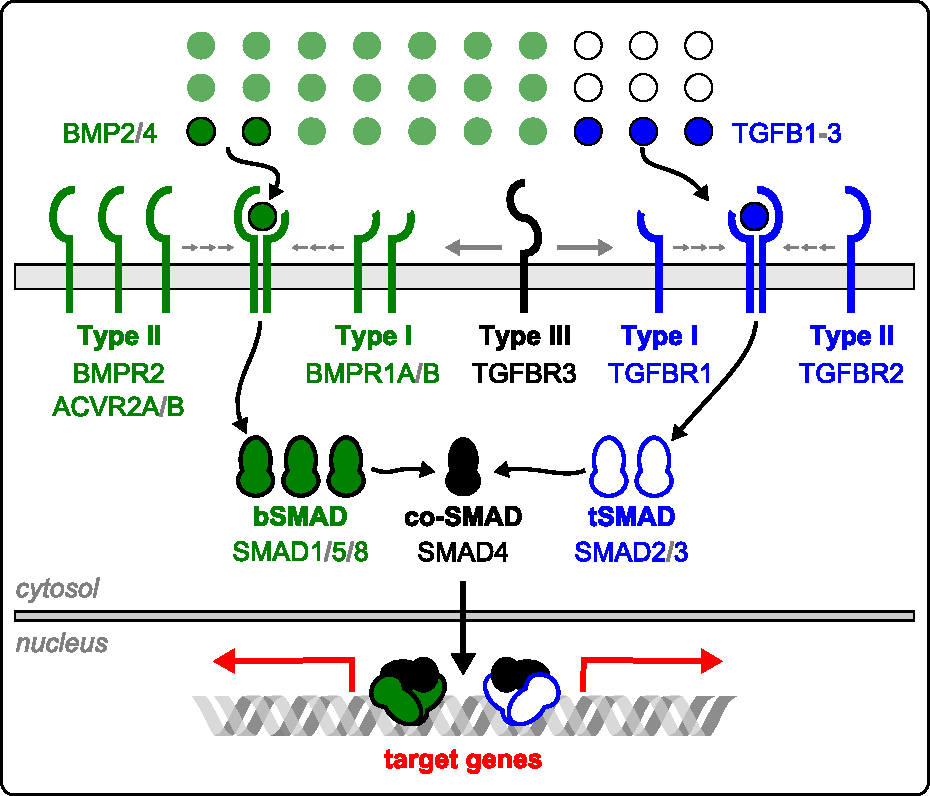
\includegraphics[width=4in]{FIGS/pathways/tgfb.pdf}
  {\singlespacing 
  \caption[Structure of the \tgfbsf\ signaling pathway]
        { Structure of the \tgfbsf\ signaling pathway.
          $\sim$30 homodimer ligands (circles) are classified into
          $\sim$20 BMPs (green), 3 \tgf s (blue), and others (outlines).
          BMP2/4 and \tgf 1-3 have distinct sets of receptors. Upon ligand
          binding, Type II receptors activate Type I receptors. In turn, active
          Type I receptors phosphorylate downstream Smads, specifically the \tgf-rSmads
		  (tSmads) or the BMP-rSmads (bSmads) (see \ar{pathways:tgfb:smads}).
		  Upon \pn\ the rSmads associate with Smad4,
          translocate to the nucleus, and bind promoters to affect transcription.
  }
  \label{fig:pathways:tgfb}}
  \end{figure}




\subsection{The \tgfbsf\ ligands}
\label{pathways:tgfb:ligands}

The more than thirty diverse ligands of the TGFB
superfamily are spread across several families,
each having a different degree of homology within their ranks
\cite{Massague2005,Ehrlich2011,Wakefield2013}. The families
include three prototypical \tgf s and
over twenty Bone Morphogenic Proteins (BMPs), as well as various Activins, Inhibins,
Growth/differentiation Factors (GDFs) and others
\cite{Massague1990,Miyazono2005,Schmierer2007}
(see the phylogenetic tree in \ar{fig:tgfb:trees}).
In this review I focus on the \tgf s and BMPs. These two families are
well-studied in the context of mammalian development and
disease and, as I describe below, they are selective for distinct receptors as well as
downstream transcription factors.


\tgfbsf\ ligands are initially made as large precursor proteins.
These precursors are cleaved intracellularly,
allowing the non-ligand portion of the precursor, the so-called
``Latency-associated peptide (LAP),'' to remain
non-covalently associated \cite{Khalil1999}. This interaction is inhibitory
and so the resulting inactive complex 
is secreted into the extracellular space.
Within this non-signaling complex resides the mature homodimeric
\tgfbsf\ ligand.


Within the mature ligand dimer, each
monomer forms a ``cysteine knot'' composed of internal
di-sulfide bridges between three cysteine-cysteine pairs.
The two monomers are covalently linked by an additional intramolecular
cysteine-cysteine bridge \cite{Nohe2004,Schmierer2007}.
The active homodimer is revealed, and then able to bind to its receptors, by separation
from the inhibitory complex. Experimentally, this
separation can be induced by various
conditions (e.g. low pH or the addition of chaotropic salts or certain proteases).
In cells, the evidence suggests that
separation is a mechanical process performed by integrins
\cite{Massague1990,Khalil1999,Shi2011}.


The three prototypical \tgf s are highly homologous,
though they have small differences in their
tertiary structures that allow for some divergence in affinities for binding partners.
\cite{Robertson2013}. For example, \tgf 2 requires a co-receptor for binding to
its cognate receptors, while \tgf 1/3 do not.
Despite these differences, the functions of the
three \tgf s are thought to be essentially the same. Therefore,
their effects in cells are expected to be a property of
\i{where} and \i{when} a member
is expressed, not \i{which} is expressed \cite{Radaev2010}.
In my own experiments, I find that
\tgf 1 and \tgf 3 do indeed produce the same phenotypic effects,
though I
observe $\sim$10-fold differences in potency between these two ligands
(data not shown).


The BMPs show a much larger degree of evolutionary diversity
than do the \tgf s, and can be broken into several
subfamilies by both homology and function (see \ar{fig:tgfb:trees}). The BMPs have
differential specificity to several receptors, and have relatively
low receptor affinity in comparison to the \tgf s (nanomolar
versus picomolar \cite{Ehrlich2011}). Along with tissue-specific 
expression patterns, this differential affinity
may account for the putative functional specificities attributed
to each BMP. Further, there are a large number of extracellular
secreted proteins that can differentially antagonize BMP signaling
(e.g. Noggin, Chordin, Gremlin, and Cerberus).


The differential receptor- and antagonist-binding affinities of
the BMPs are frequently cited as responsible for the idiosyncratic signaling outcomes
across this ligand family \cite{VonBubnoff2001,Zakin2010}. Importantly,
this is suggestive that each of these ligands may then carry the same
information. The context-dependency
may then simply stem from differences in the effective concentrations of the ligands.
There is evidence for this, since there is 
broad functional redundancy across the entire BMP family.
For example, knockout experiments in mice show that ablation of individual BMPs yields
developmental defects but only rarely lethality (BMP2/4 being the notable
exceptions) \cite{Sieber2009,Bandyopadhyay2013}. 


For simplicity, in the rest of this dissertation I focus on only one of the
BMP subfamilies. This family is composed of
BMP2 and BMP4, orthologs of \fly\ Decapentaplegic (DPP) \cite{Miyazono2005}.
This family is
highly studied in the context of mammalian stem cell differentiation and reperesents
a distinct information channel from the \tgf\ family also studied in this dissertation
(i.e. the receptors and downstream effectors are mostly non-overlapping) .


  \begin{figure}[!bt]
  \centering
  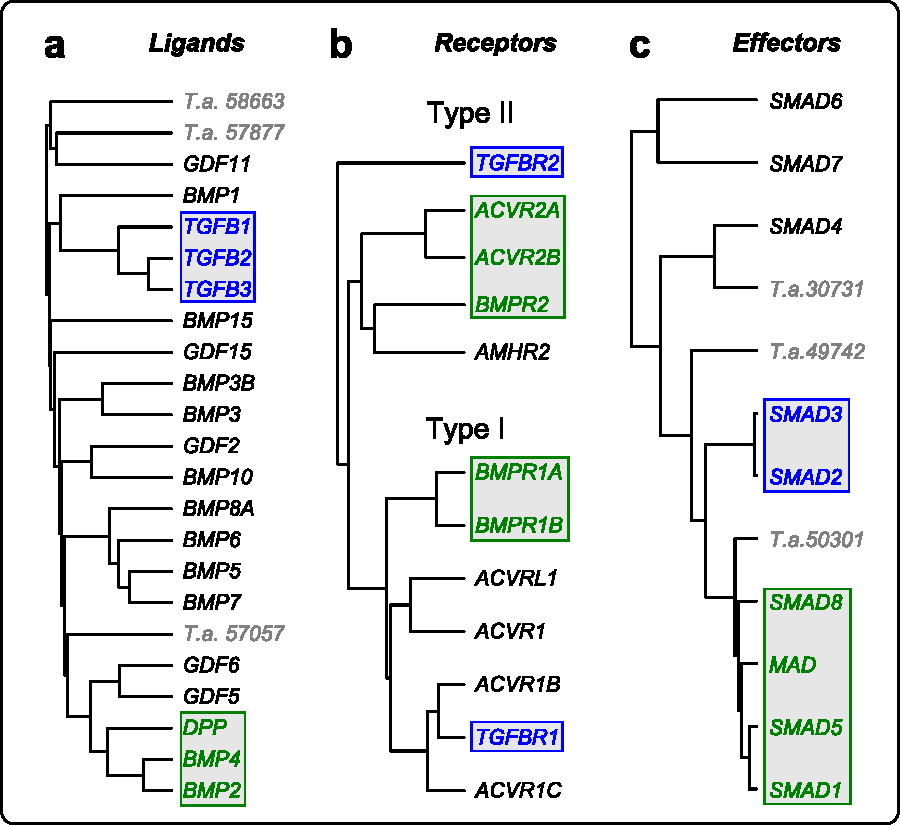
\includegraphics[width=4in]{FIGS/pathways/tgfb_tree.pdf}
  {\singlespacing 
  \caption[\tgfbsf\ phylogenetic trees]
            { Phylogeny of the \tgf\ and BMP pathway
              ligands  (\textbf{a}, \autoref{pathways:tgfb:ligands}),
              receptors (\textbf{b}, \autoref{pathways:tgfb:receptors}), and
              transcription factors (\textbf{c}, \autoref{pathways:tgfb:smads}).
              The \textit{T.a.} prefix indicates putative \ta\ proteins (gray).
			  DPP and MAD are \fly\ orthologs of BMP2/4 and Smad1/5/8.
              \tgf-specific nodes (blue) and BMP2/4-specific nodes (green) are highlighted.
              See \cite{Huminiecki2009} for a deeper discussion of the phylogeny of
              receptors and Smads in bilateria. Distances are approximate,
			  and each tree has a different scale (see \nameref{pathways:methods}).}
  \label{fig:tgfb:trees}}
  \end{figure}

    \begin{table}[!bt]
    \centering
	\footnotesize
    \caption[List of \tgfbsf\ ligands]{ Sequence sources for the 
    \tgfbsf\ ligand alignments in \ar{fig:tgfb:trees}. Note that only the 
    \tgf\ and BMP families are represented.}
    \label{table:pathways:methods:tgfbLigand}
    \begin{tabular}{lrlll}
    \hline
    Symbol & Species & & NCBI GI & Accession \\ \hline
    \tgf 1    & \i{Homo}       & \i{sapiens} & 63025222  & NP\_000651.3    \\
    \tgf 2    & \i{Homo}       & \i{sapiens} & 208022653 & NP\_001129071.1 \\
    \tgf 3    & \i{Homo}       & \i{sapiens} & 4507465   & NP\_003230.1 \\
    BMP1      & \i{Homo}       & \i{sapiens} & 4502421   & NP\_001190.1 \\
    BMP2      & \i{Homo}       & \i{sapiens} & 4557369   & NP\_001191.1    \\
    BMP3      & \i{Homo}       & \i{sapiens} & 126507087 & NP\_001192.2 \\
    BMP3B     & \i{Homo}       & \i{sapiens} & 4826740   & NP\_004953.1 \\
    BMP4      & \i{Homo}       & \i{sapiens} & 157276593 & NP\_001193.2    \\
    BMP5      & \i{Homo}       & \i{sapiens} & 10835091  & NP\_066551.1 \\
    BMP6      & \i{Homo}       & \i{sapiens} & 4502425   & NP\_001709.1 \\
    BMP7      & \i{Homo}       & \i{sapiens} & 4502427   & NP\_001710.1 \\
    BMP8A     & \i{Homo}       & \i{sapiens} & 145611428 & NP\_861525.2 \\
    BMP8B     & \i{Homo}       & \i{sapiens} & 29571106  & NP\_001711.2 \\
    BMP10     & \i{Homo}       & \i{sapiens} & 7656928   & NP\_055297.1 \\
    BMP15     & \i{Homo}       & \i{sapiens} & 257743454 & NP\_005439.2 \\
    GDF11     & \i{Homo}       & \i{sapiens} & 5031613   & NP\_005802.1 \\
    GDF2      & \i{Homo}       & \i{sapiens} & 7705308   & NP\_057288.1 \\
    GDF5      & \i{Homo}       & \i{sapiens} & 611435007 & NP\_000548.2 \\
    GDF6      & \i{Homo}       & \i{sapiens} & 48475062  & NP\_001001557.1 \\
    GDF15     & \i{Homo}       & \i{sapiens} & 153792495 & NP\_004855.2 \\
    DPP       & \i{Drosophila} & \i{melanogaster}  & 17137468  & NP\_477311.1    \\
    T.a.57057 & \i{Trichoplax} & \i{adhaerens} & 196006614 & XP\_002113173.1 \\
    T.a.58663 & \i{Trichoplax} & \i{adhaerens} & 196009532 & XP\_002114631.1 \\
    T.a.57877 & \i{Trichoplax} & \i{adhaerens} & 196008151 & XP\_002113941.1 \\
    \hline
    \end{tabular}
    \end{table}




\subsection{The \tgfbsf\ receptors}
\label{pathways:tgfb:receptors}


Receptors of morphogenic ligands must encode extracellular
ligand concentrations into some intracellular property. The \tgfbsf\ receptors
do this by converting ligand concentration into intracellular kinase activity.
Specifically, these single-pass receptors are heterodimeric
serine/threonine kinases \cite{Massague2005}.
The heterodimers consist of a Type I and a Type II
receptor that initially have no association with one another.
The two receptor types are brought together by ligand binding,
which causes a large conformational change of the receptors \cite{Hart2002}. This
conformational change is needed to bring the receptor kinase domains together,
though even after binding the receptor-receptor interactions are minimal \cite{Groppe2008}
implying a high dependence on the ligand for receptor activity.


Once brought together, the Type II receptor activates the Type I receptor by
phosphorylation. The activated Type I receptor can then, in turn, phosphorylate the
Smad transcription factors (see the pathway structure in \ar{fig:pathways:tgfb}).
Receptor activity is likely modulated, to some degree,
by endocytosis via clathrin-coated pits,
though the functional consequences of this to signaling are not well established
\cite{Derynck2003,Massague2005,Schmierer2007,Sieber2009}.


There are fewer \tgfbsf\ receptor types than there are
distinct ligands, implying that there
must be a large degree of promiscuity in receptor-ligand
binding specificity. On the other hand, the
heterodimeric nature of these receptors could in principle
generate as many distinct signaling complexes
as there are distinct \tgfbsf\ ligands,
though it is unlikely that all combinations are used in
signaling.
Indeed, both receptor types do show some degree of specificity in ligand binding \cite{Derynck2003,Dijke2004}.
The five Type II receptors and the seven type I receptors
are named after their prototypical ligands,
though the Type I receptors are commonly referred to as Activin receptor-Like Kinases (ALKs)
1-7 (see \autoref{table:pathways:methods:tgfbReceptor}).

	
	
    \begin{table}[!bt]
    \centering
	\footnotesize
    \caption[List of \tgfbsf\ receptors]{ Sequence sources for the 
    \tgfbsf\ receptor alignments in \autoref{fig:tgfb:trees}. }
    \label{table:pathways:methods:tgfbReceptor}
    \begin{tabular}{llcll}
    \hline
    Symbol   &        & Type  & NCBI GI    & Accession       \\ \hline
	TGFBR2   &        & II    & 67782326   & NP\_001020018.1 \\
	BMPR2    &        & II    & 15451916   & NP\_001195.2    \\
	ACVR2A   &        & II    & 518828583  & NP\_001265508.1 \\
	ACVR2B   &        & II    & 116734708  & NP\_001097.2    \\
	AMHR2    &        & II    & 257743467  & NP\_001158162.1 \\
	ACVRL1   & (ALK1) & I     & 116734712  & NP\_000011.2    \\
	ACVR1    & (ALK2) & I     & 4501895    & NP\_001096.1    \\
	BMPR1A   & (ALK3) & I     & 41349437   & NP\_004320.2    \\
	ACVR1B   & (ALK4) & I     & 4757720    & NP\_004293.1    \\
	TGFBR1   & (ALK5) & I     & 195963412  & NP\_001124388.1 \\
	BMPR1B   & (ALK6) & I     & 4502431    & NP\_001194.1    \\
	ACVR1C   & (ALK7) & I     & 161333835  & NP\_001104501.1 \\
    \hline
    \end{tabular}
    \end{table}


Receptor-ligand specificity is particularly sharp between the \tgf\ and BMP2/4 subfamilies
that are the focus of this dissertation: \tgf 1-3
preferentially bind to TGFBR1 (\tgf\ receptor, type 1)
and the Type II receptor TGFBR2 \cite{Inman2002}, while
BMP2/4 preferentially bind to BMPR1A/B (BMP receptor, type 1 A/B)
and the Type II receptors BMPR2 and ACVR2A/B (Activin A receptor, type 2 A/B).
\cite{Miyazono2005}. This specificity has an important consequence, that
BMP2/4 and \tgf 1-3 signaling can be considered separate information channels
at the level of receptor activation. I note however, that this separation is
not complete: cross-pathway activation has been reported in the literature
\cite{Daly2008,Goumans2003,Liu2009,Wrighton2009}
and I observe it myself (\ar{insulation:bmpTgfb}).


The channel specificity allows for the blocking of one
pathway or the other using receptor-specific inhibitors.
Several small-molecule Type I receptor inhibitors have been discovered \cite{Tojo2005,Vogt2011},
though the molecule SB431542 \cite{Inman2002} is probably the most widely used.
SB431542 specifically inhibits the Activin- and TGFB-specific Type I receptors,
and can thus be used to block TGFB signaling
while leaving BMP signaling intact. The source of specificity of this binding was demonstrated
by the structure of the TGFBR1 intracellular domain bound to SB431542. A single
amino acid difference was predicted and then experimentally shown to be able to generate a functional
but SB431542-sensitive BMPR1, or to generate a SB431542-insensitive TGFBR1 \cite{Ogunjimi2012}.


In addition to differences in receptor-ligand affinities,
further receptor-ligand specificity is gained through interactions with co-receptors.
A particularly important co-receptor, betaglycan (also called TGFBR3), increases
binding of \tgf 1/3, is required for \tgf 2 binding \cite{Derynck2003,Dijke2004}, and
also generally increases BMP signaling \cite{Kirkbride2008}. At the same time, it seems to
inhibit Activin signaling \cite{Bilandzic2011}. Betaglycan is a large protein with
$\sim$800 extracellular amino acids collectively containing two known TGFB binding
sites \cite{Kaname1996,Mendoza2009}.
It has no known intracellular signaling mechanism \cite{Bilandzic2011}, and so the
primary known role of betaglycan is to increase \tgfbsf\ ligand-receptor binding affinity.
Endoglin, a distinct co-receptor that is related to betaglycan, appears to have the opposite
role: it binds to \tgf 1/3 (not \tgf 2)
and acts negatively on TGFB signaling \cite{Lastres1996,Letamendia1998,Bernabeu2009}, though
its effects on other \tgfbsf\ members are less studied.



\subsection{The Smad transcription factors}
\label{pathways:tgfb:smads}


The information from ligand concentrations in morphogenic pathways
must be encoded by the receptors into some property of intracellular effectors.
In the case of \tgfbsf\ signaling, these effectors are the Smad
transcription factors, named after the orthologous \textit{Drosphila}
MAD protein (standing for Mothers Against DPP, DPP being
the \textit{Drosophila} BMP2/4 ortholog mentioned previously).
Ligand concentrations are believed to be encoded into Smad
nuclear concentrations and phosphorylation states.


Smads have two functional domains, the N-terminal MH1 (MAD homology 1) and the C-terminal
MH2. The MH2 domain is considerably more conserved
across the Smads. The conservation of MH2 is likely due to its
functional importance in mediating most protein-protein
interactions, though both domains have been found
to interact with various transcription factors. In particular, the C-terminus
of the MH2 domain is phosphorylated by \tgfbsf\ receptors, which creates
a binding site for Smad-Smad interactions. The MH1 domain,
on the other hand, binds DNA \cite{Derynck2003,Massague2005,Schmierer2007}.
The MH1/2 domains are connected by a linker that can be phosphorylated
by several regulatory proteins including \gsk\ (this enzyme is central
to Wnt signaling, as discussed in \ar{pathways:wnt:destruction})
and Mitogen-activated protein kinases, which typically results in Smad degradation
\cite{Fuentealba2007,Guo2008}.



There are eight mammalian Smads, Smad1-8. (The official name of Smad8 is, 
unfortunately, Smad9. I use the more common and common-sense designation Smad8
in this dissertation.) This transcription factor family
is deeply conserved and consists of several subfamilies
(see \ar{fig:tgfb:trees}), each subfamily having distinct
functions described below. In particular, Smad2/3 are nearly identical
(though Smad2 lacks a DNA binding domain),
Smad1/5/8 are quite similar to one another,
and the other Smads are considerably more diverse. Additionally,
Smad4 and Smad1/5/8 have remarkably homologous orthologs in the basal
metazoan \ta.



Functionally, the eight Smads fall into distinct groups
(see the summary \ar{table:pathways:methods:smad}): the receptor-Smads (rSmads),
the inhibitory-Smads (iSmads), and the only co-Smad, Smad4. In
brief, the functions are as follows. The rSmads are phosphorylated by the
\tgfbsf\ receptors, which creates a new binding surface for interaction with the
co-Smad. It is then the rSmads, in conjunction with Smad4, that mediate the
downstream transcriptional functions of \tgfbsf\ signaling. The iSmads, on the other hand,
contain MH2 domains and are similar in length to rSmads but lack the MH1 domain. This difference
is consistent with the primary function of the iSmads, which is to compete for interactions with
receptors, the rSmads, Smad4, and other factors. The iSmads thus behave like
dominant-negative rSmads \cite{Derynck2003}.


	
    \begin{table}[!bt]
    \centering
	\footnotesize
    \caption[List of Smads]{ Sequence sources for the 
    Smad alignments in \autoref{fig:tgfb:trees}. Abbreviations:
    rSmad = receptor-Smad, iSmad = inhibitory Smad, bSmad = 
    BMP-specific rSmad, tSmad = \tgf-specific rSmad.}
    \label{table:pathways:methods:smad}
    \begin{tabular}{llllll}
    \hline
    Symbol    & Function &         & Species & NCBI GI & Accession \\ \hline
	SMAD1     & rSmad    & (bSmad) & \textit{H. sapiens} & 51173727  & NP\_001003688.1 \\ 
	SMAD2     & rSmad    & (tSmad) & \textit{H. sapiens} & 51173730  & NP\_001003652.1 \\ 
	SMAD3     & rSmad    & (tSmad) & \textit{H. sapiens} & 223029440 & NP\_001138574.1 \\ 
	SMAD4     & co-Smad  &         & \textit{H. sapiens} & 4885457   & NP\_005350.1    \\ 
	SMAD5     & rSmad    & (bSmad) & \textit{H. sapiens} & 47778929  & NP\_001001419.1 \\ 
	SMAD6     & iSmad    &         & \textit{H. sapiens} & 218749837 & NP\_001136333.1 \\ 
	SMAD7     & iSmad    &         & \textit{H. sapiens} & 299890805 & NP\_001177750.1 \\ 
	SMAD8     & rSmad    & (bSmad) & \textit{H. sapiens} & 187828357 & NP\_001120689.1 \\ 
	MAD       & rSmad    &         & \textit{D. melanogaster} & 442625684 & NP\_001259992.1 \\ 
	T.a.50301 & unknown  &         & \textit{T. adhaerens} & 196005967 & XP\_002112850.1 \\ 
	T.a.49742 & unknown  &         & \textit{T. adhaerens} & 195998077 & XP\_002108907.1 \\ 
	T.a.30731 & unknown  &         & \textit{T. adhaerens} & 196012704 & XP\_002116214.1 \\ 
    \hline
    \end{tabular}
    \end{table}


\subsubsection{Mechanisms of Smad activity}
	
Active Smads are thought to exist as heterotrimers of two rSmads
and Smad4, though the evidence for this is indirect
except in rare cases \cite{Zieba2012}. While the simple signaling model typically
presented in the literature describes cytosolic heterotrimerization
of Smad4 and phosphorylated rSmads, followed by transport into the
nucleus, several aspects of this model either lack explicit support or are
likely incorrect.


First, it is unclear whether these
heteromeric complexes are created in the cytosol or in the nucleus,
as nuclear import of rSmads
does not require the presence of Smad4 in some cases \cite{Derynck2003}.
Further,
the rSmads and Smad4 constantly shuttle between the nucleus and cytosol
even in the absence of active signaling \cite{Nicolas2004}, 
implying that neither phosphorylation nor trimerization
are pre-requisites to nuclear localization.
Alternatively, if trimerization is required then it must be able to occur
in the absence of active signaling. In that case
it would be possible that this shuttling is allowed by transient trimerization of
inactive Smads. To my knowledge this idea has not been tested, though
an interpretation of my own results is suggestive that this may be the case \arp{insulation:bmpTgfb}.


Nuclear-cytosolic Smad shuttling was first inferred from localization
studies, from the discovery of nuclear export signals in Smad4
\cite{Pierreux2000,Watanabe2000}, and from interactions with nuclear pore
proteins \cite{Xu2002}. Shuttling was first shown directly
by the use of live-cell
experiments with exogenously-expressed fluorescent Smads \cite{Nicolas2004}.
In those experiments, photobleaching of either the nucleus
or the cytosol depleted fluorescence in both compartments over short time scales
(tens of minutes), implying that the labeled Smads were constantly
shuttling between compartments. Further, both the co-Smad and the rSmad
had significant decreases
in mobility after phosphorylation. A better model of
Smad activity, then, is that activation by the \tgfbsf\ receptors
stabilizes the nuclear fraction after import, though the mechanism
of stabilization (e.g. anchoring to nuclear proteins or reduced export rate)
is still under debate.


The dynamics of \tgfbsf\ signaling in cells have not been intensively
explored \cite{Warmflash2012}, therefore it is not known how these
dynamics vary across cell types, signaling subfamilies, or experimental conditions.
Nor is it established what the parameters are that define the kinetics (though there
have been efforts to mathematically model these pathways
\cite{Clarke2006,Umulis2009}).
There is broad consensus on the qualitative behavior of these pathways,
however. In response to a \tgfbsf\ ligand, the dimerized receptors begin
phosphorylating the rSmads. Phospho-rSmads and Smad4 then accumulate
in the nucleus, reaching saturation on the order of 40-60 minutes. 
Importantly, it is widely believed that it is the phosphorylated forms
of the rSmads that are responsible for downstream transcription, and yet
there is little direct evidence of this. The rate
of decay of nuclear localization after the peak response
seems to be highly context-dependent,
and is likely regulated in large part
by still-mysterious nuclear phosphatases that leave total protein levels
intact in the short-term (hours) \cite{Massague2012}.


Constitutive de-phosphorylation of nuclear
Smads is argued to allow for continuous re-sampling of receptor activity.
In combination with endocytosis of active receptors, this constant
re-sampling may explain the
apparent temporal ``memory'' of \tgfbsf\ signaling. For example,
washout of the ligand shortly after treatment results in a slow decay of the Smad
response while direct receptor inhbition by small molecules results in
rapid decay of the Smad signal \cite{Inman2002b}.
However, this model is somewhat inaccurate since
extracellular antagonists (such as Noggin) can more
rapidly switch off signaling than can simple removal of ligands
from the media \cite{Schmierer2007}.


\tgfbsf\ responses are also heavily regulated in the long term (hours and days)
by a number of processes that change total levels of Smads,
regulatory proteins, and other pathway components \cite{Lonn2009}.
Importantly, the \tgf\ and BMP pathways commonly upregulate their own antagonists,
the iSmads, in essentially all cell lines tested, so that
these iSmads can be considered conserved targets of \tgfbsf\ across
all or most mammalian cell types \cite{Derynck2003,Massague2012}.
(I use expression of one of the iSmads, Smad7, to confirm \tgfbsf\
pathway activity in \ar{insulation:system}.)


\subsubsection{Specificity of Smad activity}

 
\tgfbsf\ signaling through the many ligands and receptors is eventually
funneled through the five rSmads described above, representing
a dramatic collapse in the amount of potential information carried by the
large diversity of upstream components. In fact, the reduction of information content
is even more dramatic, as the rSmads are further grouped into only two
distinct information channels. I refer to these as the bSmads (BMP-responsive
rSmads) and tSmads (\tgf-responsive rSmads) as shown in
\autoref{table:pathways:methods:smad}. As a consequence of sending all
ligand stimulation through these two pathways, the cell is effectively
ignorant about which of many specific ligands has triggered an
intracellular response.


The Type I \tgfbsf\ receptors that
phosphorylate the rSmads have high specificity for either the bSmads or tSmads.
In combinatation with the receptor-ligand specificity discussed above, all
ligands eventually signal through either the tSmads or the bSmads
(though the separation is not perfect, as I observe in \ar{insulation:bmpTgfb}).
For example, the \tgf\ and Activin Type I receptors TGFBR1 and ACVR1B/C
specifically phosphorylate Smad2/3 \cite{Dijke2004}, while the BMP Type I
receptors BMPR1A/B specifically phosphorylate Smad1/5/8. This dramatic
reduction of extracellular information into only two channels is still a point of
confusion in the literature, as this idea stands opposed to broad differences in
observed consequences of \tgfbsf\ signaling, especially with respect to
effects on the transcriptional network.


As discussed in \ar{introduction:introduction}, long temporal distances between
pathway stimulation and observation of phenotypic responses make it difficult
to assign clear functional relationships between these events. This is a problem
for studies of \tgfbsf\ function, since its most highly studied outcomes are slow
processes like epithelial-to-mesenchymal transition and cellular growth arrest
and differentiation.


Adding to the complication, each rSmad has a different target DNA sequence, and binding affinity to DNA
is low for all Smads. The rSmads then have different, but overlapping, sets
of transcriptional targets
that are dramatically affected by which co-factors are present in the nucleus.
For transduced signals that carry the same information content, then, the
nucleus may use these co-factors to decide on a completely different set of outputs \cite{Massague2000}.
There are therefore only a small number of conserved transcriptional targets
for these pathways, with iSmads being perhaps the only targets present across
nearly all experimental observations \cite{Miyazono2005,Massague2012}.




\subsection{Signaling crosstalk within the TGFB superfamily}
\label{pathways:tgfb:crosstalk}

As the preceding sections show, there is a tremendous diversity of \tgfbsf\
components used throughout mammalian signaling. Importantly, it is likely
that for a given cell type, in a given \ue, there are multiple
members of each component acting at once. How cells integrate
simultaneous \tgfbsf\ signals has not been extensively
studied, though the consensus opinion seems to be that signaling crosstalk
between these pathways is mostly a product of competition for signaling components.
Given that a cell can only tell the difference between two primary arms
of \tgfbsf\ signaling, it is worth asking what information content can
exist in the combination of input signals.


Research on the problem of intra-\tgfbsf\ signaling crosstalk has been primarily performed
in developmental biology systems, especially in \textit{Xenopus laevis}. In this
system distinct \tgfbsf\ ligands set up partially overlapping gradients in portions
of the developing embryo. Experimental
manipulation of these ``morphogenetic fields'' causes \tgfbsf\ type-specific defects.
For example, Activin and BMPs have opposing roles in overlapping portions
of the embryos, so that an an artificial abundance of signaling through one pathway ablates signaling
through the other \cite{Candia1997}. The ablation occurred even when extracellular
aspects of signaling interaction were removed by expression of constitutive
receptors. It was proposed then, without explicit evidence, that the Activin/BMP cross-
inhibition could be due to competition for the co-Smad, Smad4. This claim is frequently
cited in the \tgfbsf\ literature, though to my knowledge it has not been directly
tested. In fact, my own results in \ar{insulation:bmpTgfb} suggest that the bSmads and
tSmads do not compete for the co-Smad.


Similarly, competition for receptors, co-receptors (e.g. betaglycan \cite{Bilandzic2011}
and endoglin), extracellular antagonists, and
downstream transcriptional co-factors are all cited as sources of
potential crosstalk between the \tgfbsf\ members. Such competition could be
modified by differential binding affinities of receptors to each ligand
\cite{Groppe2008,Ehrlich2011}, and thus be further amplified by differential
expression of those same receptors.
There are no well-accepted models of intra-\tgfbsf\ signaling crosstalk besides the
competition-based mechanisms above, and explicit evidence that these mechanisms
are in use by cells is currently lacking.


Finally, these pathways are also expected to cross-talk at the level of transcription,
and could do so by regulating many cellular components. Because of the high context-dependency
of target gene experession, the most obvious method of inter-\tgfbsf\ transcriptional crosstalk
is through the canonical expression of the iSmads. While expression of
these proteins will clearly inhibit \tgfbsf\ signaling, it is not at all obvious
that such a mechanism could discriminate between \tgfbsf\ family members.



\section{Review of Wnt signaling}
\label{pathways:wnt}


\subsection{Brief overview of the Wnt signaling network}

Just as with \tgfbsf, Wnt signaling is morphogenic and is deeply conserved, having
orthologs in the basal metazoan \textit{Trichoplax adhaerens} \cite{Srivastava2008}.
Also like \tgfbsf, the Wnt pathway is essential to development, results
in highly context-dependent phenotypic outcomes, and is often
disregulated in disease. In most other respects, however, these two signaling
pathways are quite different. Wnt shares no core components with the \tgfbsf\
pathway, has many more components overall (and is thus more complex), and has
different kinetics. Finally, the mechanisms of
Wnt signal transduction are less understood and more contentious than are
the mechanisms of \tgfbsf\ signaling.


The ``canonical'' Wnt signaling pathway is
shown schematically in \autoref{fig:pathways:wnt}.
This pathway consists of diverse extracellular
Wnt ligands (\autoref{pathways:wnt:wnt}) that bind to 
FZD receptors (\autoref{pathways:wnt:frizzled}) and subsequently
cause stabilization of the transcription factor \bcat\
(\autoref{pathways:wnt:bcat}). As a result, concentrations
of nuclear \bcat\ increase and this protein can then take part in
highly context-dependent changes to the cellular transcriptional
program. In addition to this canonical signaling pathway, there
are many ``non-canonical'' Wnt pathways
(as many as ten! \cite{Malhotra2009}) that are poorly understood.
My focus in this dissertation is on canonical Wnt signaling, though
I briefly review non-canonical Wnt signaling below
(\autoref{pathways:wnt:noncanon}).


I note that the term ``canonical'' is falling out of favor
in the Wnt field, so that ``canonical Wnt pathway'' is being replaced by
``Wnt/\bcat\ pathway.'' I defined the term ``canonical'' somewhat differently
in \ar{introduction:introduction} to refer to a signaling network that is
relatively distinct from other networks. Indeed, such signaling insulation
is one of the aspects of Wnt/\bcat\ signaling that has made it easier to study
than other Wnt pathways. I therefore maintain the use of ``canonical'' to
refer to the Wnt/\bcat\ pathway in this dissertation, as
it carries with it the important connotation of independence. For simplicity,
by the shorthand ``Wnt signaling'' I always refer to the canonical variant
unless otherwise specified.



  \begin{figure}[!bt]
  \centering
  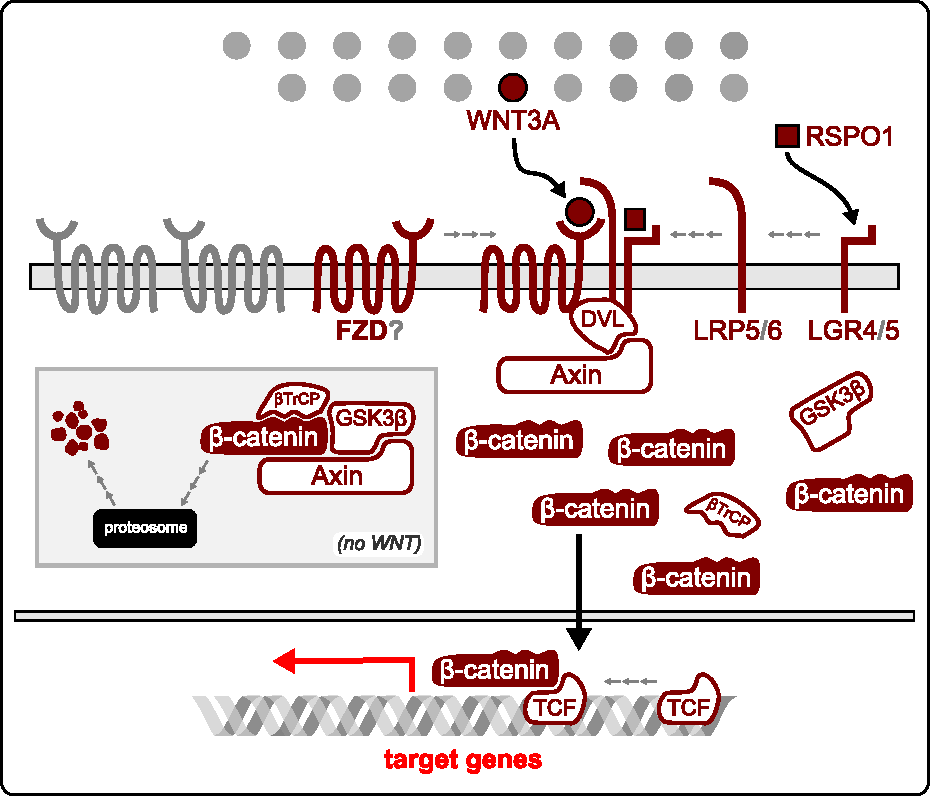
\includegraphics[width=4in]{FIGS/pathways/wnt.pdf}
  {\singlespacing 
  \caption[Structure of the canonical Wnt signaling pathway]
          {A simplified structure of the canonical Wnt signaling pathway.
          Of 19 ligands (circles), Wnt3A is the prototypical canonical ligand
          (filled red circle).
          Wnts binds to a subset of 10 FZDs, with a generally unknown degree
          of specificity. In the absence of
          Wnt (inset gray box), \bcat\ is proteosomally degraded after
          \pn\ and \ubn\ by the destruction
          complex. This complex includes the kinase \gsk, the E3 ubiquitin ligase
          \textbeta{TrCP}, and the scaffold Axin.
          In response to ligand, the destruction complex
          is disrupted in a Dishevelled (DVL)-dependent manner,
          allowing \bcat\ levels to accumulate.
          Nuclear \bcat\ binds to the co-factor TCF/Lef and together
          these factors modulate the transcriptional network of the cell.
  }
  \label{fig:pathways:wnt}}
  \end{figure}

  
  
  
  
  
\subsection{The Wnt ligands}
\label{pathways:wnt:wnt}


 \begin{figure}[!bt]
  \centering
  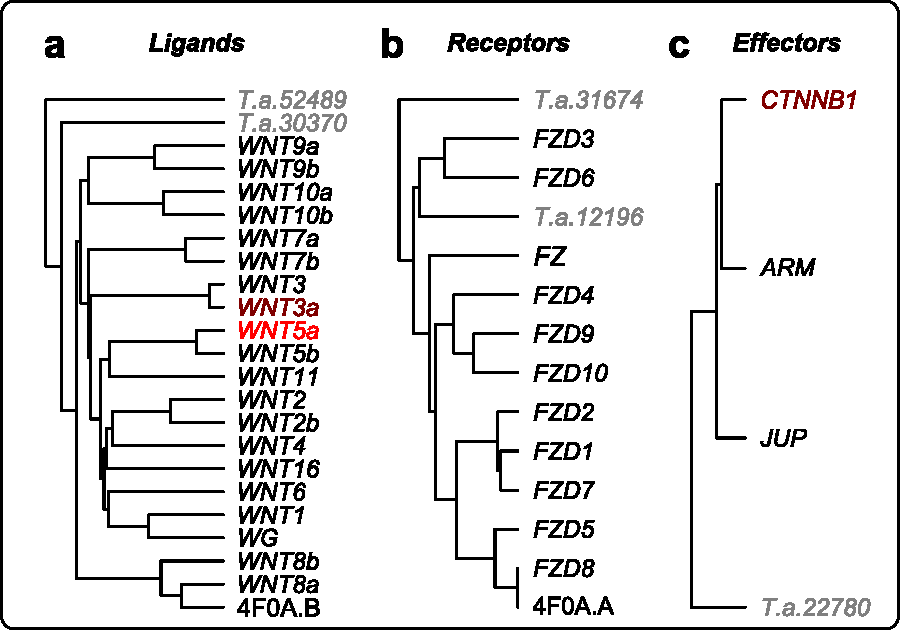
\includegraphics[width=4in]{FIGS/pathways/wnt_tree.pdf}
  {\singlespacing 
  \caption[Wnt pathway phylogenetic trees]
    { Phylogeny of the Wnt
      ligands (\textbf{a}, \autoref{pathways:wnt:wnt}),
      receptors (\textbf{b}, \autoref{pathways:wnt:frizzled}), and
      transcription factors (\textbf{c}, \autoref{pathways:wnt:bcat}).
      The \textit{T.a.} prefix indicates putative \ta\ proteins (gray).
      WG (Wingless), FZ (Frizzled), and ARM (Armadillo) are \fly\ orthologs
      of mammalian Wnt1, FZDs, and \bcat.
      JUP, Junctional Plakoglobin (also known as \textgamma-catenin)
      is a paralog of \bcat.
	  CTNNB1, gene symbol for \bcat.
      4F0A.B/A, identifiers for crystal structures of \frog\ Wnt8A
      and FZD8 used in the alignments. Wnt3A and Wnt5A (reds) are the
      prototypical canonical and non-canonical Wnt ligands, respectively. 
      As with the \tgfbsf\ pathway, note the high degree of diversity
      for each node when considering the basal \glspl{ta} proteins, and
      that the Wnts and FZDs each fall into multiple distinct subfamilies.
      Distances are approximate, in arbitrary length units
      (see \nameref{pathways:methods}).}
  \label{fig:wnt:trees}}
  \end{figure}



The mammalian Wnt ligands were initially identified with the discovery
of mouse Int-1, which was later found to be homologous to the \fly\
protein Wingless (WG). Mice are, of course,
wingless by default, and so in mammals these two gene names
were concatenated into the meaningless ``Wnt1.'' All other Wnt ligands
are named similarly \cite{Mikels2006}. In mammals, there are a total of
19 Wnts that fall into
multiple subfamilies by sequence homology (\autoref{fig:wnt:trees})
\cite{Clevers2006,Malhotra2009}. 


These small ligands ($\sim$350 amino acids) are highly cysteine-rich,
with 22 cysteine residues that have
conserved spacing across all Wnts. The evolutionary maintenance of these cysteines
was taken to imply the formation of intramolecular cysteine bridges, which suggested
that Wnt ligands should be stable proteins \cite{Mason1992}.
Further, aspects of the primary sequence, including many
charged residues, were suggestive of a protein that should be highly soluble.
Despite the expected stability and solubility of the Wnt ligands, they proved
to be quite problematic to work with \cite{Verheyen2010}.


In overexpression systems, intracellular Wnts were found to have many glycosylated forms and
tended to associate with chaperones, implying some difficulty in properly folding 
these proteins. Extracellular Wnts, in contrast, were found to have fewer glycosylated forms.
Further, the bulk of overexpressed Wnt products tended to remain in the cell \cite{Mikels2006},
and the Wnt proteins that left the cell tended to stay associated with membranes or with the
extracellular matrix \cite{Reichsman1996}. All of this data suggested that the Wnt
ligands were in fact neither stable nor soluble, explaining in part
the difficulty in purifying these proteins.


With the first successful purification of a functional Wnt in
2003, the explanation for the lack of solubility became clear: Wnts have an absolutely
conserved palmitoylated cysteine at the N-terminus. This lipidation is essential, as
mutant proteins lacking the lipidated cysteine
are incapable of signaling \cite{Willert2003}.
The relative insolubility of Wnt ligands have made them quite difficult to purify.
Indeed, purified Wnts are commercially available primarily through a single vendor
(R\&D Biosystems), and at
relatively low purity. As I show later in \autoref{insulation:system}
(\ar{fig:insulation:contamination}), this
low purity of the common reagent has important consequences to interpretation of
some experimental results.


To reduce experimental costs, studies therefore
frequently use Wnt-conditioned media instead of purified Wnts.
This approach suffers in that conditioned media contains a large amount of
unknown secreted cellular products. Cell lines that lack the Wnt
overexpression are often used as negative controls. However, given the degree of
transcriptional remodeling that the Wnt pathway can cause, there are likely
many unknown differences between Wnt-conditioned and control-conditioned
media.


The solubility problem for the Wnt ligands led to an additional difficulty,
that of determination of the tertiary structure of these proteins. Indeed, the first 
crystal structure of a Wnt was obtained only recently \cite{Janda2012}. The
primary sequence of Wnts are not related to any known protein fold, so prior
to the crystal structure there were many unknowns regarding how Wnts bind
to their various receptors and co-receptors. I touch on this more below.


    \begin{table}[!bt]
    \centering
	\footnotesize
    \caption[List of Wnt ligands]
            { Sequence sources for the 
              Wnt alignments in \autoref{fig:wnt:trees}. }
    \label{table:pathways:methods:wnt}
    \begin{tabular}{llll}
    \hline
    Symbol    & Species & NCBI GI & Accession \\ \hline
	Wnt1   & \textit{H. sapiens} & 4885655   & NP\_005421.1    \\
	Wnt2   & \textit{H. sapiens} & 4507927   & NP\_003382.1    \\
	Wnt2B  & \textit{H. sapiens} & 630044901 & NP\_001278809.1 \\
	Wnt3   & \textit{H. sapiens} & 13540477  & NP\_110380.1    \\
	Wnt3A  & \textit{H. sapiens} & 14916475  & NP\_149122.1    \\
	Wnt4   & \textit{H. sapiens} & 17402922  & NP\_110388.2    \\
	Wnt5A  & \textit{H. sapiens} & 371502087 & NP\_001243034.1 \\
	Wnt5B  & \textit{H. sapiens} & 17402919  & NP\_110402.2    \\
	Wnt6   & \textit{H. sapiens} & 16507239  & NP\_006513.1    \\
	Wnt7A  & \textit{H. sapiens} & 17505191  & NP\_004616.2    \\
	Wnt7B  & \textit{H. sapiens} & 17505193  & NP\_478679.1    \\
	Wnt8A  & \textit{H. sapiens} & 17505195  & NP\_490645.1    \\
	Wnt8B  & \textit{H. sapiens} & 110735437 & NP\_003384.2    \\
	Wnt9A  & \textit{H. sapiens} & 15082261  & NP\_003386.1    \\
	Wnt9B  & \textit{H. sapiens} & 17017976  & NP\_003387.1    \\
	Wnt10A & \textit{H. sapiens} & 16936520  & NP\_079492.2    \\
	Wnt10B & \textit{H. sapiens} & 16936522  & NP\_003385.2    \\
	Wnt11  & \textit{H. sapiens} & 17017974  & NP\_004617.2    \\
	Wnt16  & \textit{H. sapiens} & 17402914  & NP\_057171.2    \\
	WG     & \textit{D. melanogaster} & 17648113  & NP\_523502.1   \\
	T.a.30370& \textit{T. adhaerens}  & 196012489 & XP\_002116107.1 \\
	T.a.52489& \textit{T. adhaerens}  & 195996709 & XP\_002108223.1 \\ 
    \hline
    \end{tabular}
    \end{table}


	
	
	
	
	
	
\subsection{The Frizzled receptors}
\label{pathways:wnt:frizzled}



There are 10 human Wnt receptors, the Frizzleds (FZDs).
These are a diverse group of seven-pass G-coupled
protein receptors (GPCRs), though canonical signaling is mediated
primarily by non-G-protein mechanisms \cite{Angers2009}.
Upon binding to Wnt and various cofactors
the Wnt/FZD complex is likely endocytosed and
sequestered into multivesicular bodies within the cell. This receptor
internalization is essential to proper signaling
\cite{MacDonald2009,Taelman2010}. As a consequence of Wnt binding
to the Frizzled receptors, the transcription factor \bcat\
is stabilized. However, to date there are many competing
models and no clear front-runner for how FZD causes this outcome
(see \autoref{pathways:wnt:bcat}).


Essential for Wnt signaling through FZDs are the single-pass
transmembrane co-receptors, LRP5 and LRP6 (tongue-twistingly
expanding to ``Low-density lipoprotein receptor-related protein'' 5 and 6)
\cite{Clevers2006}. The ectodomain structure of LRP6 was recently
solved, revealing four tandem
beta-propellar-EGF-like domains that provide a large interface
for interacting proteins. Prior mutational studies of these domains
showed that they are essential for Wnt binding. Further, Dickkopf-1
(DKK1), a classical extracellular Wnt antagonist, was shown to bind
to these same domains, which would likely occlude the Wnt binding interface
\cite{Chen2011,Ahn2011,Cheng2011}. (I use purified DKK1 in
\ar{insulation:system} to demonstrate specificity of Wnt responses.)


Additional co-factors that are not essential but that dramatically
amplify Wnt signaling are the soluble protein R-spondin 1 (RSPO1)
\cite{Kim2005} and 
another subfamily of GPCRs, LGR4 and LGR5
(short for ``Leucine-rich repeat-containing G-protein coupled receptor
4 and 5''). It was recently discovered that these two co-factors
are themselves likely a ligand-receptor pair
\cite{Kim2005,Glinka2011,DeLau2011}, though the mechanism by which these co-factors
enhance Wnt signaling is still a mystery.


With ten receptors and multiple co-factors, we are left with the issue of
signaling specificity.
Wnts appear to have high promiscuity for the \fz s, with little
certainty in the field regarding which, if any, receptor-ligand pairings are excluded.
It is still unknown which Wnts bind to
which \fz s, or if \fz s can generally signal in both canonical and non-canonical ways
\cite{Angers2009,VanAmerongen2012}.
Unfortunately, while Wnt3A and Wnt5A are generally
considered to be the prototypical ligands for canonical and non-canonical
Wnt signaling, respectively  \cite{Huang2004}, there is
evidence that each can transduce signals through a non-prototypical pathway
under certain conditions \cite{VanAmerongen2012}.
The recent crystal structure of \frog\ Wnt8 with FZD8
did little to enhance our
understanding of the origins of receptor-ligand specificity,
as the intra-protein contacts occurred primarily at highly conserved
Wnt residues \cite{Janda2012}. This is suggestive that there is either
little specificity between ligands and receptors, or that specificity
is a more complicated outcome of interactions with other factors.




    \begin{table}[!bt]
    \centering
	\footnotesize
    \caption[List of Frizzleds]{ Sequence sources for the 
    Frizzled (FZD) alignments in \autoref{fig:wnt:trees}. }
    \label{table:pathways:methods:frizzled}
    \begin{tabular}{llll}
    \hline
    Symbol & Species & NCBI GI & Accession \\ \hline
	FZD1  & \textit{H. sapiens} & 4503825   & NP\_003496.1    \\ 
	FZD2  & \textit{H. sapiens} & 4503827   & NP\_001457.1    \\ 
	FZD3  & \textit{H. sapiens} & 8393378   & NP\_059108.1    \\ 
	FZD4  & \textit{H. sapiens} & 22547161  & NP\_036325.2    \\ 
	FZD5  & \textit{H. sapiens} & 27894385  & NP\_003459.2    \\ 
	FZD6  & \textit{H. sapiens} & 257470999 & NP\_001158087.1 \\ 
	FZD7  & \textit{H. sapiens} & 4503833   & NP\_003498.1    \\ 
	FZD8  & \textit{H. sapiens} & 13994190  & NP\_114072.1    \\ 
	FZD9  & \textit{H. sapiens} & 4503835   & NP\_003499.1    \\ 
	FZD10 & \textit{H. sapiens} & 6005762   & NP\_009128.1    \\ 
	FZ    & \textit{D. melanogaster}  & 17864440  & NP\_524812.1 \\
	T.a.12196 & \textit{T. adhaerens} & 196002269 & XP\_002111002.1 \\
	T.a.31674 & \textit{T. adhaerens} & 196014261 & XP\_002116990.1 \\
    \hline
    \end{tabular}
    \end{table}

	

\subsection{\bcat, the canonical Wnt effector}
\label{pathways:wnt:bcat}


\bcat\ is the main effector of canonical Wnt signaling. This
large protein is one of several catenins that are
used in cellular adhesion. \bcat\ itself has a large
membrane-associated pool dedicated to this task \cite{Jamieson2012}, while only a
``vanishingly small'' baseline cytosolic component is found
in Wnt un-stimulated cells \cite{Li2012}.


In the classic model of Wnt signaling, basal
\bcat\ is constitutively transcribed and translated, but then degraded
just as quickly in the absence of Wnt. Wnt stimulation stabilizes
\bcat, thus allowing cytosolic levels to build. In some systems,
cytosolic \bcat\ accumulation is measureable in as little as 15 minutes,
and reaches a stable peak response by 2 hours that can last longer
than 24 hours \cite{Li2012,Hernandez2012}.
The nuclear import/export rates for \bcat\ are unaffected by signaling,
and so it appears that nuclear accumulation resulting from Wnt 
signaling is due to an
overall change in protein abundance throughout the entire cell 
\cite{MacDonald2009,Clevers2006}.


Importantly, \bcat\ appears to encode information about extracellular
Wnt concentrations primarily in its nuclear concentration, as opposed to the
concentration of particular phosphorylation states. While various \bcat\ 
phospho-states have been discovered and claimed to
be required for the transcriptional activity of this protein, careful
quantification of post-signaling protein levels revealed that the vast
majority of \bcat\ is not phosphorylated in the presence of Wnt. Instead,
the phospho-state ends up at similar concentrations to the basal state \cite{Hernandez2012},
implying that phospho-\bcat\ does not encode Wnt ligand concentrations.


It is interesting to note that, like with the \tgfbsf\ pathways, the large
number of ligands and receptors end up bottlenecking to a small number of
effectors. This bottlenecking is more dramatic in the case of Wnt, as there
is only one \bcat\ gene to which all canonical Wnt signaling leads.
There is a highly homologous paralog, \textgamma-catenin
(also called Junctional Plakoglobin, JUP),
that differs from \bcat\ to a similar degree as does the functionally identical
\fly\ ortholog, Armadillo (see \autoref{fig:wnt:trees}). \textgamma-catenin
appears to have some functional redundancy to \bcat, and even after deletion of
both catenins some Wnt signaling has still been shown \cite{Malhotra2009}.
However, it appears that \bcat\ is the primary mediator of canonical Wnt
signaling. Interestingly, similarly to the \tgfbsf\ pathways described
earlier, this severe bottleneck implies that cells cannot
know which Wnt or Frizzled activated the pathway, unless an additional channel
of signaling carries this information.


To enact its transcriptional functions, accumulated nuclear
\bcat\ partners with one of a set of transcription
factors in the TCF/Lef family (standing for T-Cell Factor/Lymphoid 
enhancer-binding factor). There are four such proteins in mammals
that appear to be functionally redundant but do have different expression
patterns \cite{Clevers2006}. These are TCF7, TCF7L1, TCF7L2, and LEF1.
TCF1 was first discovered as a factor involved
with T-cell differentiation (hence the name) \cite{VandeWetering1991}, and later
connected to Wnt signaling after finding that a \frog\ ortholog, Xtcf-3,
could cause \bcat\ nuclear translocation \cite{MOLENAAR1996}.
TCF/Lef is normally bound to the protein Groucho, which prevents association of TCF/Lef
with \bcat. This block is lifted in response to Wnt signaling after \ubn\
of Groucho by XIAP (X-linked inhibitor of apoptosis) \cite{Hanson2012}.
It has been proposed that TCF/Lef binding to \bcat\ is stable enough to
effectively sequester it in the nucleus
and so allow for long-term Wnt signaling \cite{Jamieson2012},
though to my knowledge this has not been explicitly tested.


In complex with TCF/Lef, nuclear \bcat\ is able to bind to a diverse set of
promoters and modulate transcription. These targets are highly context-dependent,
though the negative auto-regulator Axin2 is considered to be a conserved
target of \bcat\ \cite{Clevers2006,Hatzis2008}. All canonical Wnt signals
are encoded into nuclear \bcat\ concentrations, therefore ligand-
and receptor-specific information must be lost during signal transduction.
This implies that the context-dependency of Wnt signaling responses should
be the result of transcriptional idiosyncrasies or of additional information
channels (e.g. non-canonical Wnt pathways).


\subsection{The destruction complex}
\label{pathways:wnt:destruction}


The functional effect of FZD, after binding Wnt,
is to relieve the otherwise constitutive degradation of \bcat. 
The set of proteins that are involved
with \bcat\ degradation is referred to, ominously,
as the ``destruction complex.'' The mechanisms by which this
complex degrades \bcat\ are fairly well understood, but how
active FZD causes an end to the destruction is still
highly contentious \cite{Hernandez2012,Li2012}.
Here, I discuss the components of this
complex that are best understood, and that will become important
later in the discussion on crosstalk between Wnt and \tgfbsf\
(\ar{pathways:wntTgfb:mechanism}).


\subsubsection{\gsk}

The protein Glycogen synthase kinase 3 beta (\gsk) maintains
a central role in the destruction complex. In fact, \gsk\ is
a signaling hub for many pathways, making it a prime node
for signal integration. \gsk\ is inhibited by Insulin and
growth factor signaling, which lead to phosphorylation of its N-terminal
tail. The phosphorylated tail becomes a ``pseudo-substrate'' that competes with the
actual substrates of \gsk. However, while this mechanism of inhibition
is well established, it is not clear if it is used by the Wnt
pathway. Nor is it clear whether the Wnt pathway maintains
a distinct pool of \gsk\ from growth factor pathways that can act
as an insulated information channel. If not, then modulation of a
common pool of \gsk\ by Wnt or other pathways would necessarily
create inter-pathway crosstalk.


What is clear is that this kinase requires ``priming'' phosphorylation
by another member of the \bcat\ destruction complex,
Casein Kinase 1 alpha (CK1\textalpha). This priming stems from phosphorylation 
of \bcat\ by CK1\textalpha, which produces a recognition site for subsequent
phosphorylation of \bcat\ by \gsk. Phosphorylation by
\gsk\ in turn creates a recognition site for the the ubiquitin E3 ligase
BTRC (beta-transducin repeat-containing protein, also known as \textbeta{TrCP}),
which subsequently ubiquitinates \bcat\ and sends it
off to the grinding mill of the proteosome
\cite{Frame2001,Hernandez2012}. The widely described model of
Wnt signaling has this \gsk-mediated phosphorylation being somehow
prevented in the presence of Wnt, though exactly how is a major subject of debate.
In any case, pharmacological inhibition of \gsk\ by LiCl
\cite{Stambolic1996,Hedgepeth1997} or the
ATP analog BIO \cite{Meijer2003} is sufficient to induce large increases in \bcat\ levels.
Inhibition of \gsk\ is therefore commonly used to experimentally simulate Wnt
treatment, as it gets around the earlier-mentioned difficulties
of working with purified Wnt ligands. Care should be taken when interpreting
results of these experiments, as disentangling \gsk/\bcat\ effects from the myriad of other
\gsk-mediated effects is non-trivial.


\subsubsection{Axin and APC}

There are two large proteins that act as scaffolds on which the drama
of \bcat\ destruction unfolds. These are Adenomatous
Polyposis Coli (APC) and Axin. Despite general agreement that APC is involved
in this process, its effects are often incongruous between experiments
and systems, and so there is a lack of consensus
for what APC actually does in the complex \cite{Li2012}. The roles
of Axin are better understood, and it is generally believed that
this protein forms the primary scaffold of the \bcat\ degradation
complex \cite{Roberts2012}.


Until recently, a prevailing model was that APC, which is known to
be a mobile protein, would drag the destruction complex to an unknown
subcellular compartment in order for \bcat\ degradation to occur.
However, a careful study found that APC could
effectively block Wnt signaling no matter its localization. This was
done by expressing APC constructs, modified with various localization
signals to specific compartments, in the background of APC-null cell types
\cite{Roberts2012}. All variants allowed continued \bcat\ destruction,
which convincingly disproves the APC localization model.


There exists some structural work showing the binding of APC and Axin
to one another. Intriguingly, these studies reveal that Axin binds using
a region with homology to Regulator of G-Protein Signaling (RGS)
sequences \cite{Spink2000}. Because FZDs are GPCRs (and GPCRs activate G-proteins), it is
intriguing that Axin has an RGS domain, though to my knowledge no
functional link has been demonstrated. More important is the fact that
Axin and APC appear to bind to the same interface of \bcat\ \cite{MacDonald2009},
implying that they should compete for \bcat\ binding. This is especially
important because Axin levels are widely-cited to be extremely low in cells \cite{Lee2003},
such that even a small change in its concentration (e.g. via overexpression)
would then affect the balance of APC versus Axin binding to \bcat.


\subsubsection{Dishevelled}


Immediately downstream of FZD, before the destruction complex,
is the protein Dishevelled (DVL), named
for the phenotype of the \fly\ ortholog. This component is absolutely required for
Wnt signaling in general, including non-canonical, though its precise
role is something of a mystery \cite{Angers2009,Gao2010}.
There are three paralogs in mammals, though they have a high degree
of functional redundancy and so likely differ primarily in expression pattern
(DVL1 or DVL2-null mice are viable, though
DVL3-null mice die of developmental heart defects \cite{Gao2010}).


\subsubsection{Mechanisms of destruction}


Having completed a brief tour of the destruction complex components,
I turn to the mechanisms by which Wnt signaling modulates activity of the complex.
The favored models of Wnt-induced \bcat\ stabilization involve
disabling the destruction complex so that \bcat\ phosphorylation,
and subsequent degradation, is reduced. How it does so is still contentious;
I review a few competing models below.


DVL has
a structural PDZ domain that binds to \fz, and DVL and Axin both contain
DIX domains. The homologous DIX domains of these two proteins have been proposed to
allow them to polymerize,
yielding a model wherein FZD activation pulls Axin to the membrane,
through a DVL bridge, thus disrupting the destruction complex \cite{MacDonald2009,Gao2010}.
No definitive evidence for this model has been
established, though the components can be found together in internalized endosomes during
Wnt signaling events. This suggests sequestration as a possible mechanism
for DVL-mediated Wnt signaling \cite{Angers2009}. LRP6, a Wnt co-receptor,
has been similarly proposed
to pull Axin to the membrane. This is consistent with overexpression of either DVL or an LRP6
endodomain fragment being sufficient to induce
increased \bcat\ levels \cite{MacDonald2009,Taelman2010}. This is the model
that I show in \ar{fig:pathways:wnt}.


Sequestration of the Wnt signaling complex into internal
compartments, causing isolation from interactions with cytosolic proteins
like \bcat, is a mechanism with strong support \cite{Taelman2010}.
However, there are some inconsistencies with this model. The primary
mediators of the destruction complex, Axin and \gsk, are
constitutively expressed, such that they would have to be
continuously sequestered to prevent new protein products from slowly
causing a decay in \bcat. Axin is eventually destabilized by Wnt
signaling, which gets around this caveat, but while this occurs
Axin2 levels are increased to compensate. Therefore the long-term
maintenance of Wnt activity becomes hard to explain \cite{Hernandez2012}.


Further, the key study showing this receptor-Axin complex
sequestration also found that global protein levels increased in
cells after Wnt treatment, which they interpreted to be due to
removal of a significant enough fraction of \gsk\ to also decrease its
suppression of non-Wnt proteins \cite{Taelman2010}. Given the
extremely low quantities of Axin in cells \cite{Lee2003}, and the fact
that its interaction with the much more abundant \gsk\ is stoichiometric,
it not clear how a Wnt signal could so significantly impact global
\gsk\ signaling by sequestration of the destruction complex-associated pool.
Recent work is suggestive that the global increase in protein levels
after after a Wnt response is instead due to a cell-cycle dependent
form of non-canonical signaling \cite{Acebron2014}.


In addition to the sequestration model, active
FZD complexes could negatively affect \gsk, Axin, the priming kinase CK1\textalpha,
or some combination of these. All models have support, though
the experimental bases for these models nearly universally
depend on overexpression or knockdown of pathway components \cite{Hernandez2012,Li2012}. While use of such dramatic pathway modulation
does not negate the results, it does complicate the interpretation of those results. Recent work
has begun to make use of endogenous protein levels, which has led to two strong
but incompatible models.


In the first model, the authors take an Axin-centric focus,
making the assumption that all Wnt-relevant \bcat\ destruction is mediated by
Axin \cite{Li2012}. They therefore rely on
co-immunoprecip-itation (co-IP) of endogenous Axin
for all experiments. Using this approach, they show that endogenous Axin
levels remain mostly unchanged during the early Wnt response, implying that modulation
of Axin levels is not the primary mechanism of \bcat\ stabilization
(though this does not rule out
non-degradative forms of modulation).
Instead, the authors were surprised to find that Axin pulled down minimal
\bcat\ in the absence of Wnt, and that Wnt signaling caused more \bcat\
to associate with Axin. They interpreted this to mean that interactions
on this scaffold are normally transient, but that Wnt signaling blocks
some step and so renders the destruction complex inert by saturating it
with non-transient \bcat\ binding. 
With the additional finding that Axin-bound \textbeta{TrCP}
dropped rapidly after Wnt treatment, the authors concluded that Wnt
activity somehow blocks \ubn\ of \bcat\ instead of phosphorylation.


In opposition to the saturation model, another careful study
used kinetic arguments and careful measurements of protein
quantities to show that it is indeed the \pn\ steps that control the Wnt
response \cite{Hernandez2012}. The authors start from the position that
the current models, including the saturation model, are insufficient to
explain the kinetics of the \bcat\ response to Wnt. In particular, the
models fail to explain the maintained high level of \bcat\
after $\sim$2 hours.
They show experimentally that the destruction complex is functional
whether or not Wnt is present, which directly argues against the saturation
model. Further, the authors show mathematically that a saturation-based mechanism
would have a limited range for regulation. Finally, their kinetic models
demonstrated that all observed dynamics of the pathway response could be explained
by the degree of \pn\ at two sites within \bcat. As I note in
\ar{introduction:hierarchy}, however, agreement with an abstract model
does not imply that the model is correct.


What can we make of this general confusion in the field for how Wnt
causes an increase in its effector, \bcat? First, recent studies that
focus on endogeous protein levels are clearly moving in the right
direction, and I think that the contradictions between the current
best studies will begin to be resolved by future use of similarly clean, endogenous approaches.
For my own work, I decided that it was best to avoid favoring one
model over another, since defining experiments with respect to such
tenuous models would make the future of their interpretation
uncertain. For this reason, I take a simple, mechanism-independent approach
to Wnt signaling that only requires that extracellular Wnt concentrations
are encoded as intracellular \bcat\ concentrations (\ar{insulation:introduction}).


    \begin{table}[!bt]
    \centering
	\footnotesize
    \caption[List of catenins.]{ Sequence sources for the 
    Wnt-related catenin alignments in \autoref{fig:wnt:trees}. }
    \label{table:pathways:methods:bcat}
    \begin{tabular}{lllll}
    \hline
    Symbol    & Name               & Species & NCBI GI & Accession \\ \hline
	CTNNB1    & \bcat\             & \textit{H. sapiens}      & 148233338 & NP\_001091679.1 \\
	JUP       & \textgamma-catenin & \textit{H. sapiens}      & 4504811   & NP\_002221.1    \\
	ARM       & Armadillo          & \textit{D. melanogaster} & 24639204  & NP\_476665.2    \\
	T.a.22780 &                    & \textit{T. adhaerens}    & 196000871 & XP\_002110303.1 \\
    \hline
    \end{tabular}
    \end{table}

    

    
\subsection{Non-canonical Wnt signaling}
\label{pathways:wnt:noncanon}


Our understanding of the
best-understood Wnt signaling pathway, the canonical pathway, is still
incomplete. The various non-canonical Wnt signaling
pathways are even less understood. This in large part because the readouts
of these pathways
are either hard to measure or are affected by other factors whose contributions are
difficult to disentangle \cite{Angers2009,VanAmerongen2012}.
Though the focus of this dissertation is on canonical signaling, here I briefly
review the non-canonical pathways to provide background for
an instance of inter-pathway crossalk between \tgfbsf\
and non-canonical Wnt5A signaling.


There are many different non-canonical pathways, with some authors counting
up to ten \cite{Malhotra2009}, though the true number is
certainly unknown. Perhaps the best-studied non-canonical
pathways are those of Planar Cell Polarity (PCP) and Convergent Extension (CE) in \fly.
However, it is important to note that these pathways are studied in different
systems (the wing and developing embryos, respectively)
and share core components, so it is unclear how distinct these pathways truly
are \cite{VanAmerongen2012}. This ambiguity is common among the non-canonical pathways. An additional
non-canonical pathway studied in mammalian systems activates
Ca$^{2+}$ signaling, though the consequences of such
signaling are mostly unknown \cite{De2011}.


While the mechanisms, readouts, and functional consequences of non-canonical signaling
are poorly understood, there are several key components that are well-established.
At the level of receptors, ROR2 (expanding to ``Receptor tyrosine kinase-like
orphan receptor'') has an extracellular Wnt-binding domain homologous to
that of FZD. This receptor activates Ca$^{2+}$ signaling in response
to Wnt5A. The ROR2 homolog ROR1 also has this domain,
but may be a pseudo-kinase \cite{VanAmerongen2012}.
Importantly, Wnt5A signaling through ROR2 is well established to inhibit long-term
canonical Wnt/\bcat\ signaling, though how it does so is still unknown
\cite{Huang2004,Angers2009,Malhotra2009,VanAmerongen2012}.


Downstream of the receptors, DVL is frequently (but not always) 
required for non-canonical signaling. Interestingly, DVL seems to use different
protein domains for canonical and non-canonical signaling, so that mutation of
one domain can preferentially block one type of signaling \cite{Gao2010,VanAmerongen2012}.


Finally, there is no good reason to believe that canonical and
non-canonical signaling must occur in isolation. Because of the
promiscuity of Wnt-FZD binding and the unknown contribution of each
FZD to the various Wnt signaling pathways, it is reasonable to
expect that a Wnt signal may trigger multiple simultaneous downstream pathways.
Perhaps this is a mechanism by which the cell obtains more information
about the original signal, since \bcat\ concentrations alone can only encode
information about the overall extent of canonical Wnt activity, not which 
Wnts triggered that activity.

\section{Functional importance of \tgfbsf\ and Wnt signal integration}
\label{pathways:wntTgfb:function}


Having covered the canonical \tgfbsf\ and Wnt signaling pathways, we
can now move forward to the topic of this dissertation: inter-pathway crosstalk.
The goal of this section is to both motivate the study of Wnt/\tgfbsf\
crosstalk and to review the work that has been done in this field.
There are many systems in which both of these pathways are intensively
studied (indeed entire
textbooks have been written on these pathways). However, most of this work
studies each pathway indepenently; there exists a much
smaller body of work on Wnt/\tgfbsf\ inter-pathway
crosstalk. One of the more experimentally-tractable of such systems is the
adult mammalian gut, and so I focus my review on this system.


The study of adult stem cells has advanced rapidly in recent years,
especially with the identification of resident stem cells for several
tissues \cite{Barker2010} and with the discovery that differentiated
cells can be turned pluripotent by expression of a handful of
transcription factors \cite{Takahashi2006}.
However, there is still much that we do not understand about stem
cell biology in general, especially because \i{in vitro} studies
are difficult to map back to \i{in vivo} phenomena,
and because each stem cell system has proven to have its own quirks including
differential use the same genetic pathways.


In particular, work in this field has
pointed toward \tgfbsf\ signaling being a major factor in stem cell
differentiation, while canonical Wnt signaling seems to control stem cell
maintenance. There are cases where this oppositional role assignment does not occur
\cite{VonBubnoff2001,Fischer2002,Nakashima2005,Itasaki2010a,
Feigenson2011,Lander2012,Malhotra2009,Davidson2012}, though
it is fairly common across stem cell systems
\cite{Verheyen2010,Libusova2010,Gregorieff2005,VandeWetering2002,
Schepers2012,Teo2006}. These roles are
particularly well-studied in the context of the mammalian intestine.


Our understanding
of the intestinal stem cell system has increased significantly in recent years,
due in no small part to the work of Hans Clevers and colleagues.
Clevers' group has dissected the function of many genes involved with
intestinal stem cell development (with a focus on canonical Wnt), has
unambiguously identified the stem-cell population \cite{Barker2007a},
and has developed an \textit{in vitro} system for culturing intestinal
stem cells in such a way that they behave like homoestatic \textit{in vivo} crypts
\cite{Sato2011a,Sato2011b}. This work has even led to successful engraftment
of intestinal stem cells isolated from one mouse into the damaged
intestine of another \cite{Yui2012}. Given the potential value to stem
cell therapy, and the connection of stem cells with colon cancer
\cite{Zeki2007,Barker2009a}, a deeper understanding of intestinal stem
cells is highly sought after in hopes of obtaining new therapeutic strategies
for many bowel diseases.


While the gut stem cell system is highly studied, it is poorly understood
how intestinal stem cells
integrate distinct signals from their environment, such as Wnt and \tgfbsf,
and thus choose one of several differentiated outcomes. Given the oppositional
roles of \tgfbsf\ and Wnt in the gut, and their various functional interactions in other systems
\cite{Attisano2004,Labbe2007,Chong2009,Itasaki2010a,Minoo2010a,
Serra2011,Feigenson2011,Rodriguez-Carballo2011,Chen2012a,Akhmetshina2012,Song2014},
it is important to understand generally how cells integrate these two signals.


\subsection{\tgfbsf\ and Wnt in the intestinal crypt}
\label{pathways:wntTgfb:gut}

\subsubsection{Crypts are the functional unit of intestinal epithelium}

The small and large intestine both contain
similar stem cell systems. Between these two organs, morphological
differences in stem cell systems are revealing in terms of the distinct organ functions.
The small intestine contains a high fraction of absorptive cells (enterocytes)
and an increased epithelial surface area due to relatively large lumenal projections termed
villi, consistent with its role in digestion and absorption of food.
The colon is predominantly made up of mucus-secreting goblet cells
and completely lacks villi, consistent with its need to carry potentially
abrasive and toxic waste \cite{Iacopetta2002}. The protective role of
goblet cells is highlighted by the connection between goblet cell
loss and rapid tumor formation in mice \cite{Yang2008}. The colon is of
particular clinical interest due to the high rates of cancer
and inflammatory diseases of this organ \cite{Jemal2010}. Despite macroscopic differences
in morphology, many aspects of of the stem cell biology seem to be similar
in the small and large intestine.


A cross-section of the intestine would reveal a hollow tube whose wall
consists of several tissue layers. The
most-lumenal layer consists of the mucosa, a single sheet of epithelium
over stromal tissue (fibroblasts, collagen, blood/lymphatic vessels, etc.),
together forming crypts and their support structures.
The epithelium sits atop a basement membrane
\cite{Simon-Assmann2010} which in turn is immediately adjacent to
myofibroblasts such that each crypt is essentially sheathed in these cells.
Though it is likely that important signaling takes place between the
epithelium and stroma \cite{Simon-Assmann2010,Kosinski2010,Ingham2011},
these signals are difficult to study and their importance is unclear given
the fact that \i{ex vivo} isolated crypts maintain a differentiating,
homeostatic structure even in the
absence of a macroscopically polarized stroma \cite{Sato2011a,Lahar2011}.


The crypts are the functional unit of the intestine. The single epithelial layer
of each crypt contains only
$\sim$10 stem cells at the base that divide on average once per day,
generating a conveyor belt of rapidly dividing and differentiating cells
\cite{Snippert2010} \arp{fig:pathways:crypt}. These ``transit amplifying'' cells stop dividing
after full differentiation and are eventually lost to the lumen of the gut
\cite{Eisenhoffer2012}. This process is fast, such that the entire non-stem
cell population of a crypt is turned over every 3-5 days \cite{Buske2011}.


In the small intestine, the top of the crypt (which is the base of
the villus) is roughly the point at which cells are completely differentiated.
Note that this generally accepted model of crypt turnover
is based on studies of the small intestine and is thought to be similar in
the colon, though there are important
differences between the organs that should be considered.
For example, the large intestine completely lacks the paneth cells that have
recently been reported to be required for stem cell maintenance in the small
bowel. However, colonic crypts do contain cells
expressing similar surface proteins \cite{Sato2011b}.
Additionally, the entirety of the colonic crypt contains apparently-differentiated
cells, suggesting that the transit amplifying population
is much smaller than in the small bowel.
On the other hand, the literature generally supports that the population
dynamics and signaling factors are similar between the small and large
intestine, and between mouse and human.


	\begin{figure}%[ht]
	\centering
	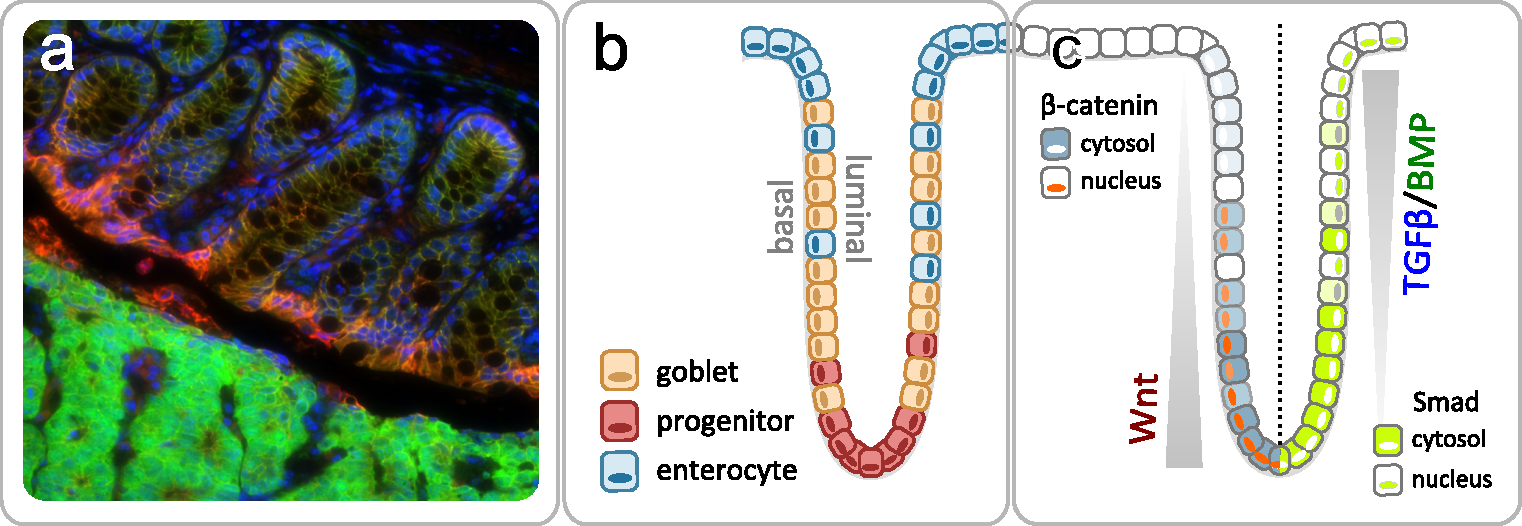
\includegraphics[width=6in]{FIGS/pathways/crypt.pdf}
	{\singlespacing 
	\caption[Expression patterns of Wnt and \tgfbsf\ in colonic crypts]
            { Overview of \tgfbsf\ and Wnt signaling patterns
            in the colonic crypt. \b{a}, Immunostained crypts
            from a CPC;APC mouse \cite{Hinoi2007} showing two opposing sides pinched
            together, with the dark lumen in between. Blue, DNA; green,
            \bcat, red, E-cadherin. The bottom set of crypts are tumorous;
            note the global increase in \bcat. Image curtesy Michael
            Ramirez and Curtis Thorne (Altschuler \& Wu lab,
            Univeristy of Texas Southwestern).
            \b{b}, Cartoon of colonic crypt
            structure, showing key cell types. \b{c}, Cartoon of
            signaling gradients in the crypt, showing high Wnt
            at the crypt base and high \tgfbsf\ at the crypt tops.}
	\label{fig:pathways:crypt}}
	\end{figure}



\subsubsection{Opposing gradients of \tgfbsf\ and Wnt in crypts}


Within the crypt epithelium, there are distinct patterns of expression for
the Wnts and the \tgfbsf\ ligands that together seem to control cell
fate in a crypt-axis positional manner. Using fluorescence in situ hybridization
(FISH), Clevers' group showed that canonical Wnts and various FZDs were
preferentially expressed in the crypt base, while non-canonical Wnts were
expressed throughout the crypt or only at the top \cite{Gregorieff2005}.
The same group later found that LGR5, a Wnt co-receptor,
is a highly specific marker for intestinal stem cells \cite{Barker2007a}.
This discovery allowed for labeling and purification of this cellular population,
and the demonstration that this cell type alone could
re-create crypt-like structure \i{in vitro}.


There is evidence that the paneth cell population is the source
of canonical Wnt3A in the crypt base \cite{Sato2011b},
though this is confounded by a study showing that this cell
type can be ablated \textit{in vivo} without loss of stem cell maintentance
\cite{Rizk2012}.
In contrast to canonical Wnt, but similarly to non-canonical Wnt,
\tgfbsf\ ligands and receptors are expressed exclusively in the
the differentiated epithelium at the tops of the crypts
\cite{Hardwick2004,Massague1990}
and villi \cite{Yamada2013}. Smad activity is restricted to
the same parts of the crypt \cite{Hardwick2008,Libusova2010}.


How the gradients are established and maintained, especially in the face
of a constanty turning over cell population, is not well understood.
The relatively long lifespans of the paneth cell population
\cite{DeSantaBarbara2003} hint that this
cell type may serve as a sort of anchor for these gradients. Another
potential source of gradient maintenance are the transmembrane ephrin
receptors and their ligands, which seem to be required for proper cell sorting: their
loss results in disorganized cellular positions within colonic crypts.
Intriguingly, these ephrins and receptors are regulated by canonical Wnt signaling,
though how these two phenomena interact is unclear \cite{Batlle2002}.


Importantly, it is unclear whether these gradients actually function as such.
While the gradients could be formed by secreted molecules diffusing over
multiple cell lengths, the relative insolubility of Wnts argues against this.
Indeed, in the developing fly wing and in the vertebrate notochord, there is
recent evidence that diffusion of Wnt is not the mechanism by which it creates
gradients \cite{Alexandre2014,Serralbo2014}. Additionally, because Wnt and \tgfbsf\
have so many extracellular antagonists, the presence of a ligand gradient is neither
required nor sufficient to have a functional gradient \cite{Wakefield2013}.


\subsection{Wnt drives stem cell maintenance; \tgfbsf\ drives differentiation}

While the opposing gradients of these two pathways hint at
opposing functional roles, they do not imply it. 
The gradients could be a macroscopic consequence of cell sorting.
Or, the gradients could be a marker of crypt position without exerting any
concentration-dependent influence.
The biological argument that most favors truly oppositional roles is that
modulation of one pathway, experimentally or in the context of disease,
is generally paired with opposite deviations of the other pathway.
I reviews examples of this below.


\subsubsection{Increased Wnt signaling is a driver of colon cancer}

It is well established, and has been for some time, that over-activation of
canonical Wnt is a primary force in colon cancer. Multiple components of
the pathway have been implicated in this disease, though clearly some of
the signaling nodes are easier to hijack than others. One could imagine
upregulation of Wnts, receptors, or \bcat\ as possible
mechanisms. However, the pathway
has negative feedback, via \bcat-mediated expression of Axin2, and 
so constitutive upstream activity would be insufficient for maintenance of
high \bcat. Therefore constitutively high \bcat\
activation is more easily obtained by blocking the function of the destruction complex.
Perhaps for this reason, the most commonly modulated signaling
nodes are components of the complex itself. There is at least one example
of receptor-level modulation, however, which is that RSPO1
(the soluble Wnt co-factor) is frequently
upregulated in colon cancer due to genomic translocation \cite{Seshagiri2012}. Whether this
upregulation is functionally important to cancer, however, is still speculative.


By far, the most common Wnt pathway modification in colon cancer is mutation
of APC, the destruction complex component with perhaps the most mysterious functional role.
In fact, APC is nearly always mutated in this type of cancer ($>$80\% of cases)
\cite{He1998,Clevers2006,Roberts2012}. Interestingly, APC is rarely completely lost,
instead being frequently truncated to its
N-terminal half. The reason for this truncation preference
is unclear and has been the cause of much speculation \cite{MacDonald2009}.
However, it is worth noting that there need not be a reason.
Perhaps there are more ways to mutate APC such that it is truncated instead
of ablated, in which case truncation would simply be the more likely
evolutionary step. However, there is some cell culture evidence that APC-truncated
and APC-null cells have different phenotypes, especially with respect to cell
adhesion and migration \cite{Burgess2011}.


While it is not clear what exactly APC is doing in the destruction complex,
the effects of APC loss on Wnt signaling are well-established.
APC knockdown results in rapid nuclear accumulation of \bcat, followed by increasingly
dense cell packing due to overgrowth and then, eventually, a less-differentiated
cellular phenotype \cite{Sansom2004}. Remarkably,
stem cell-specific deletion of APC leads to adenoma formation
in mere days and results in macroscopic tumor development in only 3-5 weeks
\cite{Barker2009a}. Importantly, this effect requires
\bcat-dependent expression of Myc \cite{He1998},
a classic oncogene, as ablation of Myc can rescue the APC mutant phenotype \cite{Sansom2007}.


\subsubsection{Decreased \tgfbsf\ is a driver of crypt dysplasia} 


Given my earlier description of the \tgfbsf\ pathways as inducers of differentiation,
it is perhaps no surprise that these pathways tend to be lost in colon cancer
and in other dysplastic diseases. As with the Wnt pathway, certain components of the
\tgfbsf\ pathways are more prone to being hijacked by disease than others.
Loss of any particular \tgfbsf\ ligand would likely be insufficient to ablate pathway
activity, as would loss of several of the receptors, given the redundancy at this
level of signal transduction. The obvious targets then are the Smads, which are indeed
mutated or lost in the context of several dysplasias.


Of the Smads, the most efficient target of ablation in disease would be Smad4,
since it is the bottleneck for all upstream \tgfbsf\
pathways. Indeed, Smad4 is commonly mutated in colon cancer ($>$15\% of cases) and
in pancreatic cancer ($>$50\% of cases) \cite{Levy2005,Seshagiri2012}. Additionally, next-generation
sequencing of $>$70 human colon tumors revealed a high prevalence of Smad2 (one
of the \tgf-specific rSmads)
mutations \cite{Seshagiri2012},
allowing speculation on the importance of \tgf\ signaling in colon cancer.
In another dysplastic
disease, Juvenile Polyposis, BMP signaling loss is found in $>$50\% of cases
\cite{Haramis2004a,Miyazono2005,Hardwick2008}. Though it is unknown if the BMP loss in
these cases was sufficient
to cause the human phenotype, overexpression of the BMP-inhibitor Noggin
is sufficient to generate ectopic crypts within the villi of mouse models \cite{Haramis2004a}.


The above data suggest that gain of Wnt signaling has a more potent effect
than does loss of \tgfbsf\ signaling, at least in the context of colon cancer.
However, changes to one of these pathways is always accompanied by changes in the other.
For example, BMP signaling has been found to be reduced
in $>$70\% of colon cancers \cite{Hardwick2008}, though only $\sim$15\% of cases
have mutations in the pathway. Further, in a study of microarrays from 250
colorectal tumor samples it was found that Smad4 and
\bcat\ levels were generally anti-correlated
\cite{Freeman2012}. Taken together, these correlative
results are suggestive that these two pathways
are in some way regulating one another, and that for Wnt signaling to become
tumorigenic it has to suppress the
\tgfbsf-mediated drive towards cellular differentiation.



\section{Nodes of crosstalk between \tgfbsf\ and Wnt}
\label{pathways:wntTgfb:mechanism}


In this dissertation I am interested in understanding the inter-pathway
crosstalk between \tgfbsf\ and Wnt. As discussed in \ar{introduction:encoding},
one of the most problematic aspects of studying cell signaling
is the determination of which input signals a cell cares about
and into what intracellular property that information is encoded.
As this chapter has so far detailed, the field consensus for both
\tgfbsf\ and Wnt is that it is the concentration of the ligands
that carries the information that cells care about
(these are morphogenic signals) and this
information is encoded into nuclear concentrations of canonical
transcription factors.


Further, the literature reviewed in the previous section
strongly suggest that the \tgfbsf\ and Wnt
pathways have many opportunities for crosstalk, especially in the
mammalian gut. With established input/output relationships
in hand, and reason to suspect that the pathways in question modulate one
another, we can begin to ask how these pathways integrate information.
This section provides a review of the signaling nodes at which
inter-pathway crosstalk is thought to occur (see the graphical
summary in \ar{fig:pathways:xtalk}).




  \begin{figure}[!bt]
  \centering
  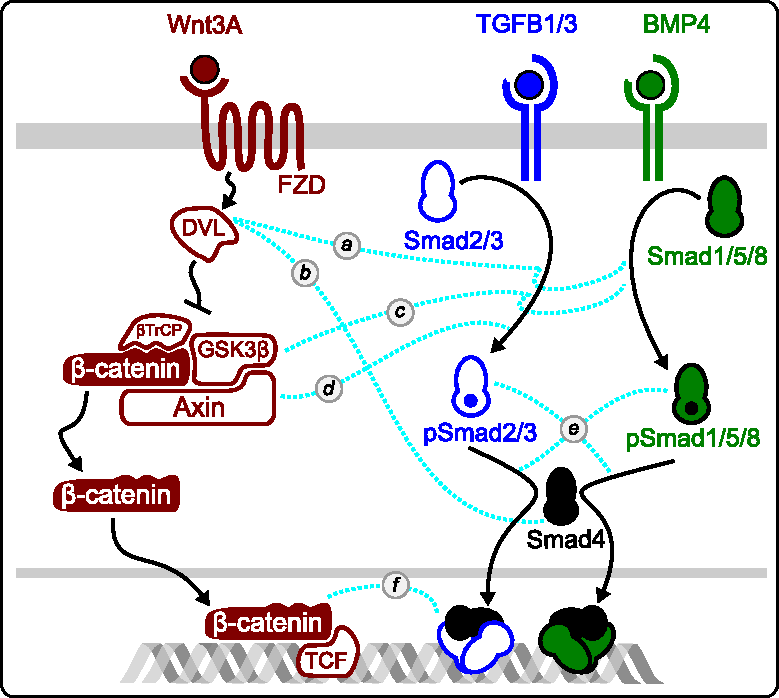
\includegraphics[width=4in]{FIGS/pathways/tgfb_wnt_xtalk.pdf}
  {\singlespacing 
  \caption[Overview of Wnt and \tgfbsf\ pathway crosstalk]
        { Overview
          of Wnt and \tgfbsf\ pathway crosstalk. 
          This dissertation focuses on canonical Wnt, BMP, and \tgf\, as mediated by Wnt3A,
          BMP4, and \tgf 1/3. Dashed lines indicate
          literature-established
          links between pathways. References:
          \textit{a}\cite{Warner2003,Warner2005a,Liu2006};
          \textit{b}\cite{Mamidi2012};
          \textit{c}\cite{Fuentealba2007,Guo2008};
          \textit{d}\cite{Furuhashi2001,Guo2008,Liu2006b};
          \textit{e}\cite{Candia1997};
          \textit{f}\cite{Zeng2008}.}
  \label{fig:pathways:xtalk}}
  \end{figure}




\subsection{Smad and DVL}
\label{pathways:wntTgfb:dvl}

The DVL proteins, being key post-receptor mediators
of both canonical and non-canonical signaling, occupy
an important position for potential crosstalk with
the \tgfbsf\ pathway. Interactions of DVL with
the MH2 domain of Smads were first identified in a yeast two-hybrid
screen \cite{Warner2003}. The same group and others confirmed
the possibility of such interactions in mammalian cells using
co-immunoprecipitation (co-IP) after overexpression of Smads, with the
conclusion that all three DVLs could bind to most of the
Smads (\ar{fig:pathways:xtalk}a) \cite{Warner2003,Warner2005a,Liu2006}. The Smad-DVL
interaction was also shown for non-canonical Wnt signaling,
with a downstream mediator of Wnt5A, PAR1B, precipitating with both
Smad and DVL (\ar{fig:pathways:xtalk}b) \cite{Mamidi2012}.


While co-IP of overexpressed proteins shows the possibility of interaction,
they neither guarantee that it occurs under normal conditions
nor imply that the interaction has a functional outcome.
In some of the studies cited above, attempts were made
to demonstrate functional consequences of Smad-DVL interaction.
This was done by treating cells with ligands for one or both
pathways after ablation or overexpression of other signaling components.
Using this approach, it was found that BMP2 treatment
could increase complexed DVL1/Smad1, while
Wnt3A-conditioned media had the opposite effect \cite{Liu2006},
suggesting that pathway interactions are sensitive to signaling activity.
Additionally, RNAi of
all three DVLs, PAR1B, or ROR2 can attenuate TGFB signaling, while
overexpression of DVL3 or FZD2 can enhance it
\cite{Mamidi2012,Miyoshi2012}.
The authors of these studies interpreted the data to mean that the
\tgfbsf\ pathway is directly modulated by the Wnt pathways during
signal transduction, though the mechanisms are unclear and seemingly
complex. Importantly, the observed cross-pathway modulation seemed to be mediated
by interactions between DVL and Smad.


A functional consequence of TGFB and non-canonical Wnt5A
integration was recently reported in the context of wounded
colonic epithelium \cite{Miyoshi2012}. In that study, the
authors found that mice lacking Wnt5A were less able to repair
colonic epithelial lesions, seemingly due to an inability of
progenitor cells to differentiate in the wound. Given the use of
\tgfbsf\ pathways in gut stem cell differentiation, it is perhaps
unsurprising that the authors could link a \tgf\ signaling
deficiency to this Wnt5A phenotype. Specifically, they
found that treatment of \textit{ex vivo} colonic
crypts with high concentrations of Wnt5A yielded downstream
\tgf\ responses. The mechanisms for this were not clear, except
for a dependence on the TGFBR2 and ROR2 receptors, but are
consistent with DVL-mediated interactions. Importantly, my
own work is suggestive that this Wnt5A/\tgf\ connection is due to an artifact
(\ar{insulation:system}).


\subsection{Smad and Axin}
\label{pathways:wntTgfb:axin}


Axin, being a large protein that is central
to canonical Wnt signaling, is another good candidate
for interactions with \tgfbsf\ components
(\ar{fig:pathways:xtalk}d). Indeed,
in a co-overexpression assay of Axin and Smad3,
the two proteins were found to co-IP. This interaction was
dependent upon a region of Axin between the \bcat\ and
DVL binding domains, though how binding to this site
might affect Wnt signaling is unclear.
Further, \tgf\ responsiveness was
increased when Axin was overexpressed \cite{Furuhashi2001}.
This was interpreted to mean that Axin can stabilize
Smad activity, either by preventing Smad degradation or
by blocking some other form of Smad interference. 


Two additional studies looked into the consequences
of Smad-Axin interactions, but with contradictory results.
In one case, Axin was found
to bind to an iSmad (Smad7) and to mediate degradation
of that Smad by Arkadia, an E3 ubiquitin ligase. As
a consequence, overexpression of both Axin and Arkadia
led to enhanced TGFB signaling \cite{Liu2006b}. While
the outcome is the same as that described above, the
mechanism is essentially the opposite. In
a different study, Axin was again found to destabilize
a Smad, but this time an rSmad via \gsk\
instead of an iSmad via \ubn. As a result, TGFB signaling was instead
attenuated by increased Axin, and
Axin depletion by RNAi amplified TGFB signaling \cite{Guo2008}.


How can we make sense of the studies of Axin-Smad
interaction, that are all mutually incompatible? It is important
here to recall that basal Axin levels in cells are extremely
low \cite{Lee2003}. Because this protein acts as a scaffold,
its overexpression can have a few obvious non-physiological
effects. The first is that Axin is a big protein, with many
binding surfaces, and so the observed Smad-Axin interactions
may be due to what would normally be extremely rare binding
events. The other is that while Smad and Axin may interact,
overexpression of the scaffold causes interactions between Smad and other
Axin-bound proteins to become at first enhanced and then diluted
as the amount of Axin increases. All of the cited studies use
Axin overexpression, and so the apparent contradictions between them
may be due to either of these phenomena.



\subsubsection{Smad and \gsk}
\label{pathways:wntTgfb:gsk}

\gsk, which primes \bcat\ for \ubn, is able to phosphorylate a large
fraction of the proteome. Recently, this was found include the bSmads
(experimentally) and the tSmads (based on computational prediction).
The Smads have a canonical \gsk\ recognition sequence in the linker region
between the functional MH1 and MH2 domains. Phosphorylation of these sites
in bSmads was found to be \gsk-dependent and could be 
down-regulated by Wnt3A treatment (\ar{fig:pathways:xtalk}c). Importantly, the study
found that total Smad levels were not affected by Wnt treatment, but
that the active phospho-state did show measurable decreases \cite{Fuentealba2007}.
This data was therefore interpreted to mean that \gsk\ could modulate
the long-term duration of Smad activity.


\subsubsection{Smad and \bcat}
\label{pathways:wntTgfb:bcat}


Finally, we turn to interactions with the final effector of
the Wnt pathway, \bcat\ (\ar{fig:pathways:xtalk}f).
Like Axin, the large size of \bcat\ provides
many potential binding interfaces. Additionally, its role as the bottleneck
of all canonical Wnt signaling makes it a good candidate for
cross-pathway interaction. Even so, evidence for interactions between
Smad and \bcat\ are quite limited. There is some evidence that
\fly\ MAD and Armadillo (Smad and \bcat\ orthologs) compete with one another
for binding to TCF, such
that DPP (the BMP2/4 ortholog) can cause a downstream block of \bcat\ transcriptional output
\cite{Zeng2008}. Similarly, though with different functional consequences, in mammals
an iSmad (Smad7) can co-IP with \bcat\ and overexpressed TCF/Lef \cite{Edlund2005}.
It is therefore unclear whether a Smad/\bcat\ interaction is important to signaling
through either pathway.


  
\subsubsection{Transcriptional crosstalk}
\label{pathways:wntTgfb:transcription}


The nodes of putative crosstalk described above occur prior to transcription
factor entry into the nucleus. I therefore classify these as nodes of 
``signaling crosstalk.'' What about at the level of transcription,
after the nucleus has received the transcription factor output of each signaling pathway?
Our knowledge of \tgfbsf/Wnt crosstalk is almost entirely due to studies
at this level of interaction, however studies that look at both pathways
simultaneously are rare. Instead, transcriptional crosstalk is often inferred
by studies finding that activity of one pathway
modulates transcriptional output commonly associated with the other.


A few direct crosstalk studies have been performed, though their results
are not easily comparable.
In the case of TGFB and Wnt, activation of both pathways was found to
increase output of a Wnt transcriptional reporter. The lack of
Smad-response elements in this promoter suggested that
the co-activation was due to an interaction occurring prior to promoter
binding \cite{Warner2005,Lei2004}. Microarrays
from similar co-treatment experiments showed that a set of genes
were regulated differently in the context of both inputs than with either
input alone, though no obvious patterns were found (e.g. genes that
were increased by Wnt or TGFB were not necessarily further increased by both)
\cite{Warner2011,Labbe2007}.


Transcriptional crosstalk is most frequently inferred by the presence
of consensus binding motifs for \bcat/TCF and the Smads within the
same target gene promoter. In this way, 
instances of direct transcriptional co-regulation by TGFB/Wnt
have been found in several systems 
\cite{Hussein2003,Zhou2012,Labbe2000,Rodriguez-Carballo2011}.
For the focal case of the gut in this section, the
co-regulation of the Myc promoter by these two sets of transcription factors
is of obvious relevance \cite{Hu2005} .



\section{Discussion}
\label{pathways:discussion}

The preceding chapter provided a glimpse of the complexity and uncertainty
in the properties of Wnt and \tgfbsf\ signaling and inter-pathway crosstalk.
Here, I summarize the salient points that lead to the approaches and hypotheses
of my experimental work in \ar{insulation:introduction}.


\subsection{Wnt and \tgfbsf\ use morphogenic encoding systems}

The consensus in the literature is that Wnt and \tgfbsf\ signaling are
morphogenic, meaning that they encode information about ligand concentrations.
As I have noted throughout this text, the fact that these pathways
yield concentration-dependent effects does not imply that this is the only
information about the signals that cells are using.


In
\ar{imaging:information} I discuss how the information content
of biological outputs can be quantified using the mutual information metric.
Published reports indicate that the information content of many biological
input/output relationships, when measured by imaging,
is quite low \cite{Cheong2011}. My own
measurements, using the careful image correction discussed in 
\ar{imaging:introduction}, yield only slightly higher information content.
This low mutual information between ligand concentrations and the
outputs of signaling imply that cells can only effectively determine
whether a signal is present or not; they cannot determine a precise
absolute concentration. In effect, these morphogens are not
morphogenic at the single-cell level!
This limited information content of the concentration-based encoding system is
especially interesting in light of the dramatic network
bottlenecking of both pathways. Together, the implication is that
cells can neither determine which of many
different ligands is present in the environment nor the precise concentrations of those
ligands. How much information about these pathways, then, do single
cells have access to?


On the other hand, we may be neglecting additional information channels
that cells use to encode more accurate models of their extracellular
environments. ``Non-canonical'' information channels may provide
just such content. Or, just like the fly embryo syncytium that
makes use of multiple noisy
transcription factor gradients to obtain accurate positional
information (see \ar{introduction:encoding}) \cite{Gregor2007,Dubuis2011},
cellularized systems such as the intestinal crypt may integrate Wnt and \tgfbsf\
concentrations in order to more accurately define fates or positions along
the crypt axis.


\subsection{Signaling crosstalk reduces information content}


In the preceding sections and in my primary experimental work in
\ar{insulation:introduction}, I take care to classify pathway crosstalk
into distinct types: pre-nuclear signaling crosstalk versus nuclear
crosstalk at the level of transcription.
This is for an important reason, which is that
integrating pathways at the level of signal transduction
causes a loss of information content available to the nucleus.
In other words, the nucleus loses
knowledge about the environment when pathways intersect during signaling.


As an example, the cell makes an internal model of environmental \tgfbsf\
using concentrations of active Smad.
If \tgfbsf\ were the only thing that could activate Smad, then the cell
would ``know'' that \tgfbsf\ was present in the environment any time that
active Smad levels increased. But what if Wnt could also modulate Smad?
In this case, when the nucleus sees changes to active Smad levels, it cannot
know whether \tgfbsf, Wnt, or some combination of the two ligands are
present in the environment. This contrasts to the case where \tgfbsf\
ligands only modulate Smad, and Wnt only modulates \bcat, so that the
internal model within the cell models the more complex
reality of the external environment.


\subsection{Informational asymmetry between the cell and its environment}


Perhaps cells only need limited information about their environments,
such that the reduction of information caused by complex inter-pathway
processing during signal transduction is of no consequence. This would
be surprising, however, as these very same cells are what create the
information-rich extracellular milieu in the first place
(e.g. by secreting signals and otherwise modifying the environments of their
neighbors). How could information-poor
intracellular networks create information-rich extracellular environments?


One possibility is that each cell type present in a complex environment
does indeed have limited information about that environment. It could
then be the case that the environmental complexity is
simply due to the combination of low-information outputs from many distinct cell types.
In effect, individual cell types would be insulated from the complexity
of their environments, and would only have to worry about processing the
few signals that they are capable of ``understanding.''


\subsection{Uncertainty in the nodes of \tgfbsf/Wnt signaling crosstalk}


Crosstalk at the level of signaling reduces what a cell can know about
its environment. It is therefore important to determine whether such crosstalk
truly exists before speculating on why a cell would need so little
environmental information, as I so prematurely began to do above.


Cellular signaling is extremely difficult to study, for the reasons
outlined in \ar{introduction:introduction}, and the studies
cited in the current chapter are illustrative of this fact.
While it is possible that the results of all of the cited studies are accurate,
they must be interpreted with care. In particular, all of the cited
studies that identified nodes of \tgfbsf/Wnt crosstalk relied on
some combination of overexpression, RNAi knockdown, or pharmacological
inhibition of pathway components. All of these methods can push the
global cellular signaling network into states that normal cells
cannot inhabit. This is especially true for studies involving
\bcat\ and Axin, as these proteins are scaffolds that are normally present at extremely
low concentrations.


Also, the further apart experimental inputs and outputs
are in time, the less accurate our inferences can be about the mechanisms
connecting them. The cited studies rely heavily on co-immunoprecipitation of
overexpressed pathway components to demonstrate the possibility of
interactions. They then use transcriptional reporters
and other long-term readouts to measure the consequences of these interactions.
However, a relationship between physical interactions
and downstream consequences can only be demonstrated by specifically blocking
that interaction. This has not been done for any node of
putative \tgfbsf/Wnt signaling crosstalk, and for good reason: such an
experiment is exceedingly difficult to design.


In short, current studies on \tgfbsf/Wnt signaling crosstalk do not
show either that such crosstalk definitively exists, nor that the crosstalk
has functional consequences if it does exist.
Indeed, in \ar{insulation:introduction} I show strong evidence under
endogenous signaling conditions that
these pathways are insulated from one another during signaling. This
implies that nuclei maintain more accurate models of their environments by
integrating \tgfbsf\ and Wnt primarily at the level of transcription.


It will be important for future studies to accurately
determine the information content of the \tgfbsf\ and Wnt signaling pathways,
and how that information is encoded by the cell. 
Such studies may reveal that cells encode more about the signal than
just its concentration.
In combination with the results of \ar{insulation:introduction},
that the integration of these
pathways gives cells more information, we may find that
cells create more accurate internal models of their extracellular
environments than is currently believed.



\section{Methods}
\label{pathways:methods}


    \begin{table}[!bt]
    \centering
	\footnotesize
    \caption[List of crystal structures used in phylogenetic trees.]
    { Sources of structures used in
    alignments for \autoref{fig:tgfb:trees} and
	\autoref{fig:wnt:trees}. }
    \label{table:pathways:methods:ligandStruct}
    \begin{tabular}{lllc}
    \hline
    Symbol  & Species & PBD ID & Source \\
    \hline
    TGFB1 &  \textit{Homo sapiens}   & 3KFD.A  & \cite{Radaev2010}  \\
    TGFB2 &  \textit{Homo sapiens}   & 2TGI.A  & \cite{Daopin1992}  \\
    TGFB3 &  \textit{Homo sapiens}   & 2PJY.A  & \cite{Groppe2008}  \\
    BMP2  &  \textit{Homo sapiens}   & 1REW.A  & \cite{Keller2004}  \\
	SMAD3 &  \textit{Homo sapiens}   & 1U7F.A  & \cite{Chacko2004}  \\
	SMAD4 &  \textit{Homo sapiens}   & 1U7F.B  & \cite{Chacko2004}  \\
	SMAD7 &  \textit{Homo sapiens}   & 3KMP.A  & \cite{BabuRajendran2010}  \\
	Wnt8  &  \textit{Xenopus laevis} & 4F0A.B  & \cite{Janda2012} \\
	Fz8   &  \textit{Xenopus laevis} & 4F0A.A  & \cite{Janda2012} \\
    \hline
    \end{tabular}
    \end{table}
    

\textbf{Sequence alignments.}
I obtained sequence data from the National Center for Bioinformatics (NCBI)
servers, choosing each time
the top listed isoform from the Genes database
Protein structures are from the
Research Collaboratory for Structural Bioinformatics (RCSB)
protein database (PDB) \arp{table:pathways:methods:ligandStruct}.
I used subsets of these sequences and structures for alignment in
Promals3D \cite{Pei2008} to obtain phylogenetic trees.
This multi-sequence alignment algorithm takes advantage of
structural information for improved alignments, however the
distances in the phylogenies should be considered approximate since the method
for calculating genetic distance is more naive than the alignment method.
The crystal structures were included in the Wnt and Frizzled trees
because of species differences from the primary sequence data.
Structures for the \tgfbsf\ and Smad trees were dropped because
their sequences identically match a subset of the primary sequences.
The trees were drawn with the R package `ape' \cite{Paradis2004}.


For predicting \textit{Trichoplax adhaerens} orthologs of
genes, I used PSI-BLAST \cite{Altschul1997} with some combination of
human and \i{Drosophila melanogaster} reference proteins. I ran one or more
iterations of the algorithm on the seed sequences, and then chose the few top hits
that were dramatically better matches by both query coverage
and identity. Each putative \ta\ ortholog is listed in the appropriate table in
this chapter. These orthologs are in agreement with the literature
\cite{Srivastava2008}.


Specifically, to identify \tgf/BMP
orthologs I used the \tgf 1-3, BMP2/4, and DPP sequences as seeds,
resulting in 3 putative orthologs (>50\% coverage). For the TGFB receptors, I used
the Type I and Type II receptors separately, but each yielded
a large number (>200) of putative matches that had reasonable identity
(>30\%) but low coverage (<50\%) or vice versa. I therefore did not
include these in the phylogenetic tree. For the Smads,
I used the eight human genes and the \fly\ MAD as seeds, yielding three good hits
(>90\% coverage, >30\% identity). For the Wnts, I used all 19 human
genes and fly WG, yielding 2 hits ($\geq$68\% coverage, >30\% identity).
For the Frizzleds, I used all 10 human
genes and fly FZ, yielding 2 hits (>50\% coverage, $\geq$30\% identity).
For \bcat\ I used human CTNNB1 with Junctional Plakoglobin (JUP, also known
as gamma-catenin) and fly arm,
yielding 1 hit (>70\% coverage, >70\% identity).




